% Konfigurationsdatei f\"ur die Pfaddefinitionen einlesen
%  se-wa-pfade.tex
%
%
%  J\"org Baumgart
%  2012-12-20
%  
%  Pfaddefinitionen (Ordnerdefinitionen) f\"ur das Einlesen von
%  -- .sty-Dateien und
%  -- Textbaustenen f\"ur die Hinweise zur Verwendung von LaTeX
%  -- jpg-Bildern
%
\newcommand{\seWaPathSty}{se-wa-styles}
\newcommand{\seWaPathText}{se-wa-textbausteine-vorlagen}
\newcommand{\seWaPathJpg}{se-wa-jpg}

%
%
% Festlegung der Sprache:
\newcommand{\seWaSprache}{deutsch}
%\newcommand{\seWaSprache}{englisch}

%
% Einlesen der .sty-Dateien
%
%  se-wa-input-styles-v096.tex
%
%  Joerg Baumgart 01.08.2011
%
%  Zusammenfassung und Konfiguration wichtiger Styles f\"ur die 
%  Erzeugung von Seminar-, Projekt- und Bachelorarbeiten
%
%  2012-03-12: auf Version 0.94 umgestellt
%
%
% 2012-12-13: auf Version 0.95 umgestellt
%                     Sprachoptionen englisch/deutsch zusammengef\"uhrt
%                     bchart.sty hinzugenommen
%                 
%
% 2013-01-27: auf Version 0.96 umgestellt
%                     algorithm2e-Paket integriert
%
%
% 2013-07-08: auf Version 0.97 umgstellt 
%                     utf8, Fehlerkorrekturen bei pa1
%
% 2014-02-02: auf Version 0.971 umgestellt
%                     Workaround für Fehler im KOMAScript 3.2
%                     KOMAoption listof un documentclass übernommen
%
%
%
%


\documentclass[12pt,BCOR=10mm,headinclude=on,footinclude=off,bibliography=totoc,listof=ignorechapter]{scrreprt}
\usepackage[T1]{fontenc}
\usepackage[utf8]{inputenc}
\usepackage{ifthen}
% 2012-12-13
\ifthenelse{\equal{\seWaSprache}{deutsch}}{% Deutsche Einstellungen
\usepackage[ngerman]{babel}% 
}{% Englische Einstellungen
\usepackage[english]{babel}% 
}

\usepackage{lmodern}

\usepackage{tikz} % Graphikpaket, das zu pdfLaTeX kompatibel ist
\usepackage{xkeyval} % Definition von Kommandos mit mehreren optionalen Argumenten
\usepackage{listings} % Formatierung von Programmlistings
\usepackage{graphicx} % Einbinden von Graphiken
\usepackage{color}
\usepackage{\seWaPathSty/slashbox} % Diagonalen in Tabellenfeldern
\usepackage{framed} % Erzeugung schwarzer Linien am linken Rand zur Hervorhebung von Textteilen
\usepackage{caption} % Korrektes Setzen einer mehrzeiligen float-Unterschrift bei neu definierten float-Umgebungen
\usepackage{floatrow}
% 2012-12-13
\usepackage{\seWaPathSty/bchart} % Kommandos zur Erzeugung von Balkendiagrammen
% 2013-01-27 
\usepackage[boxed,ngerman]{\seWaPathSty/algorithm2e}
%\usepackage[tworuled,vlined,ngerman]{\seWaPathSty/algorithm2e}


% Es wird jeweils die sty-Datei importiert und entsprechende Konfigurationseinstellungen werden vorgenommen

\usepackage{\seWaPathSty/se-jb-scrpage2} % Formatierung der Kopf- und Fu{\ss}zeilen
\usepackage{\seWaPathSty/se-jb-footmisc}    % Fussnoten besser formatieren

\usepackage{\seWaPathSty/se-jb-glossaries-v097} % Abk\"urzungsverzeichnis, Symbolverzeichnis, Glossar
   
\usepackage{\seWaPathSty/se-jb-floatrow}    % Definition und Konfiguration von float-Umgebungen (figure, table, die neue programm-Umgebung)
% Achtung: se-jb-varioref muss nach se-jb-floatrow importiert werden; 
% andernfalls ist der counter programm f\"ur die labelformat-Anweisung noch nicht definiert   
\usepackage{\seWaPathSty/se-jb-varioref-v097}   % Definition von Querverweisen
\usepackage{\seWaPathSty/se-jb-chngcntr}   % Kapitelweise oder globale Nummerierung von Abbildungen etc.
   
\usepackage{\seWaPathSty/se-jb-listen} % Definition neuer, besser formatierter Listen
% 2014-02-02
%\usepackage{\seWaPathSty/se-jb-kommandos-v097} % neue Kommandos f\"ur Seminar-, Projekt- und Bachelorarbeiten
\usepackage{\seWaPathSty/se-jb-kommandos-v0971} % neue Kommandos f\"ur Seminar-, Projekt- und Bachelorarbeiten
% 2012-12-13
\ifthenelse{\equal{\seWaSprache}{englisch}}{\usepackage{\seWaPathSty/se-jb-kommandos-englisch-v097}}{}


%
% Individuelle Konfiguration des Dokumentes
%
%  Individuelle Konfiguration einer Projektarbeit/Bachelorarbeit
%
%
%
%

% 2012-10-27
%
% \"Anderung des Schrifttyps f\"ur das gesamte Dokument
%
% Das gesamte Dokument wird in einer serifenlosen Schrift gesetzt
%\renewcommand{\familydefault}{\sfdefault}
%
% Das gesamte Dokument wird in einer Serifenschrift gesetzt
% Achtung: serifenlose Schriften sind jetzt grunds\"atzlich nicht mehr nutzbar!
%
%\renewcommand{\sffamily}{\normalfont}

% 2012-12-05
%
% Verwendung des url-Pakets
% Durch den optionalen Paremeter hyphens wird eine Trennung 
% von URLs auch nach Bindestrichen erlaubt
\usepackage[hyphens]{url}


% 2012-10-27
%
%
% Literaturverzeichnis
% 
% Literaturverzeichnis gem\"ass den Vorgaben von Theisen aufbauen
\usepackage{\seWaPathSty/se-jb-jurabib-theisen} 
% Verwendung der Harvard-Zitierweise
%\usepackage{\seWaPathSty/se-jb-jurabib-harvard} 

% Weitere Optionseinstellungen f\"ur das Koma-Script
%
% Zwischen Abs\"atzen einen Abstand von 0.5 \baselineskip erzeugen
\KOMAoption{parskip}{full}
%
% Vergleiche Duden "Gliederung von Nummern, S.111" 
% DIN 5008 anschauen, wenn sie neu ver\"offentlicht wurde
\KOMAoption{numbers}{noendperiod}
%
%



%  Voreinstellungen f\"ur floats
%  Durch die verwendeten Parameter wird die Wahrscheinlichkeit deutlich kleiner, 
%  dass Gleitobjekte (z. B. Abbildungen) ans Ende des Dokumentes verschoben 
%  werden; 
%  Achtung: clearpage erzwingt die Ausgabe von Gleitobjekten
%
\renewcommand{\topfraction}{1}  % Gleitobjekte d\"urfen eine Seite zu 100% belegen 
\renewcommand{\bottomfraction}{1} % Entsprechender Wert f\"ur den unteren Teil der Seite
\renewcommand{\textfraction}{0} % Eine Seite darf auch ohne Fliesstext existieren
%%%\renewcommand{\floatpagefraction}{1} % Bedeutung unklar, daher keine Ver\"anderung des Vorgabewertes 
                                                                        % von 0.5; eventuell bringt ein \"Anderung auf 1 etwas, wenn 
                                                                         % Probleme mit floats auftreten
                                                                         
                                                                         
                                                                         
% Konfiguration von Programm-Listings
% 
% Achtung: hier gibt es nahezu beliebig viele weitere Konfigurationm\"oglichkeiten; vgl. Paketdokumentation
%
\lstset{language=Java,basicstyle=\ttfamily,keywordstyle=\color{blue},captionpos=b,aboveskip=0mm,belowskip=0mm,
          xleftmargin=0em}               
          
%
% Grundkonfiguration der Abs\"ande zwischen den Items der maximal f\"unf Verschachtelungsebenen der 
% neuen Listenumgebungen
%                                                                             
% Initialisierung der Abst\"ande zwischen den items f\"ur seList; Grundeinheit: 0.5\baselineskip; siehe se-jb-listen
\seSetlistbaselineskip{1}{0.75}{0.75}{0.75}{0.75}
% Initialisierung der Abst\"ande zwischen den items f\"ur seToplist; Grundeinheit: 0.5\baselineskip; siehe se-jb-listen
\seSettoplistbaselineskip{1}{0.75}{0.75}{0.75}{0.75}     


% Einlesen der sprachabh\"angigen Konfigurationsdatei
%
%
\ifthenelse{\equal{\seWaSprache}{deutsch}}{% deutsch
% wa-konfiguration-deutsch
%
% 2012-12-13
% 
% Diese Datei wird f\"ur die Sprachoption deutsch verwendet, d. h.  
% \newcommand{\seWaSprache}{deutsch}
%
%
% In dieser Datei k\"onnen Neudefinitionen vorgenommen werden f\"ur:
% -- Verzeichnisse
% -- Unter-/\"Uberschriften von Abbildungen, Tabellen und Listings
% -- Querverweise innerhalb des Textes

% 2013-01-26: Konfiguration des Algorithmenverzeichnis
%
%
%

% 2013-07-08: Querverweis auf Anhang hinzugenommen
%
%
%


%
%  Konfiguration der verschiedenen Verzeichnisse
%
%  abstandEintrag: Wert wird mit \baselineskip multipliziert
%

%
%  Abbildungsverzeichnis
%
\seKonfigurationAbb[
%verzeichnisname=Abbildungsverzeichnis,
labeltextLinks=, % kein Text links;
%labeltextRechts=:,
labelbreite=1cm,
%labeleinzug=1cm,
%abstandEintrag=1,
%newpage=ja,
%pnumwidth=20mm,
%dotsep=1000,
%tocrmarg=4.5cm,
%abstandVerzeichnis=-1mm
]

%
% LIstingverzeichnis
%
\seKonfigurationPrg[
%verzeichnisname=Listing-Verzeichnis,
labeltextLinks=,
%labeltextRechts=:,
labelbreite=1cm,
%labeleinzug=2cm,
%abstandEintrag=1,
%newpage=ja,
%pnumwidth=20mm,
%dotsep=1000,
%tocrmarg=4.5cm,
%abstandVerzeichnis=-10mm
]

% 2013-01-26
%
% Algorithmenverzeichnis
%
\seKonfigurationAlg[
%verzeichnisname=Algorithmen-Verzeichnis,
labeltextLinks=,
%labeltextRechts=:,
labelbreite=1cm,
%labeleinzug=2cm,
%abstandEintrag=1,
%newpage=ja,
%pnumwidth=20mm,
%dotsep=1000,
%tocrmarg=4.5cm,
%abstandVerzeichnis=-10mm
]




%
% Tabellenverzeichnis
%
\seKonfigurationTab[
%verzeichnisname=Liste der Tabellen,
labeltextLinks=,
%labeltextRechts=:,
labelbreite=1cm,
%labeleinzug=0.5cm,
%abstandEintrag=1,
%newpage=ja,
%pnumwidth=20mm,
%dotsep=1000,
%tocrmarg=4.5cm,
%abstandVerzeichnis=-10mm
]

%
% Abk\"urzungsverzeichnis
%
\seKonfigurationAbk[
%verzeichnisname=Liste der Abk\"urzungen,
%labelbreite=3cm,
%labeleinzug=0.5cm,
%abstandEintrag=1,
%newpage=ja,
%abstandVerzeichnis=-10mm
]

%
% Symbolverzeichnis
% 
\seKonfigurationSym[
%verzeichnisname=Liste der Symbole,
%labelbreite=4cm,
%labeleinzug=3.5cm,
%abstandEintrag=1,
%newpage=ja,
%abstandVerzeichnis=-10mm
]

%
% Glossar
%
\seKonfigurationGlo[
%verzeichnisname=Glossar,
%abstandEintrag=0,
]



% (eventuelle) Neudefinition f\"ur die Unter-/\"Uberschriften von Abbildungen, Tabellen und Listings
%
%
%\renewcommand{\seCaptionNameAbbildung}{Abb.}
%\renewcommand{\seCaptionNameTabelle}{Tab.}
%\renewcommand{\seCaptionNameProgramm}{Prg.}


% % (eventuelle) Neudefinition f\"ur Querverweise innerhalb des Textes
%
%
%
%\renewcommand{\seQuerverweisSeite}{Seite}
%\renewcommand{\seQuerverweisAbbildung}{Abb.}
%\renewcommand{\seQuerverweisTabelle}{Tab.}
%\renewcommand{\seQuerverweisProgramm}{Prg.}
%\renewcommand{\seQuerverweisGleichung}{Gl.}
%\renewcommand{\seQuerverweisAlgorithmus}{Alg.}
%
\renewcommand{\seQuerverweisChapter}{Kapitel}
% 2013-07-08
\renewcommand{\seQuerverweisAppendix}{Anhang}
\renewcommand{\seQuerverweisSection}{Kapitel}
\renewcommand{\seQuerverweisSubsection}{Kapitel}
\renewcommand{\seQuerverweisSubsubsection}{Kapitel}
\renewcommand{\seQuerverweisParagraph}{Kapitel}


%
% Kommandos f\"ur die Konfiguration von URL-Eintr\"agen im Literaturverzeichnis
%
\renewcommand*{\biburlprefix}{\jblangle{}URL: }
\renewcommand*{\biburlsuffix}{\jbrangle{}}
\renewcommand*{\bibbudcsep}{ -- }
\AddTo\bibsgerman{\renewcommand*{\urldatecomment}{Zugriff am }}


%
}{% englisch
% wa-konfiguration-englisch
%
% 2012-12-13
% 
% Diese Datei wird f\"ur die Sprachoption englisch verwendet, d. h.  
% \newcommand{\seWaSprache}{englisch}
%
%
% In dieser Datei k\"onnen Neudefinitionen vorgenommen werden f\"ur:
% -- Verzeichnisse
% -- Unter-/\"Uberschriften von Abbildungen, Tabellen und Listings
% -- Querverweise innerhalb des Textes

% 2013-07-08: Querverweis auf Anhang hinzugenommen
%
%
%


%
%  Konfiguration der verschiedenen Verzeichnisse
%
%  abstandEintrag: Wert wird mit \baselineskip multipliziert
%

%
%  Abbildungsverzeichnis
%
\seKonfigurationAbb[
verzeichnisname=List of Figures,
labeltextLinks=, % kein Text links;
%labeltextRechts=:,
labelbreite=1cm,
%labeleinzug=1cm,
%abstandEintrag=1,
%newpage=ja,
%pnumwidth=20mm,
%dotsep=1000,
%tocrmarg=4.5cm,
%abstandVerzeichnis=-1mm
]

%
% LIstingverzeichnis
%
\seKonfigurationPrg[
verzeichnisname=List of Program Listings,
labeltextLinks=,
%labeltextRechts=:,
labelbreite=1cm,
%labeleinzug=2cm,
%abstandEintrag=1,
%newpage=ja,
%%pnumwidth=20mm,
%dotsep=1000,
%tocrmarg=4.5cm,
%abstandVerzeichnis=-10mm
]


% 2013-01-26
%
% Algorithmenverzeichnis
%
\seKonfigurationAlg[
verzeichnisname=List of Algorithms,
labeltextLinks=,
%labeltextRechts=:,
labelbreite=1cm,
%labeleinzug=2cm,
%abstandEintrag=1,
%newpage=ja,
%pnumwidth=20mm,
%dotsep=1000,
%tocrmarg=4.5cm,
%abstandVerzeichnis=-10mm
]


%
% Tabellenverzeichnis
%
\seKonfigurationTab[
verzeichnisname=List of Tables,
labeltextLinks=,
%labeltextRechts=:,
labelbreite=1cm,
%labeleinzug=0.5cm,
%abstandEintrag=1,
%newpage=ja,
%pnumwidth=20mm,
%dotsep=1000,
%tocrmarg=4.5cm,
%abstandVerzeichnis=-10mm
]

%
% Abk\"urzungsverzeichnis
%
\seKonfigurationAbk[
verzeichnisname=List of Abbreviations,
%labelbreite=3cm,
%labeleinzug=0.5cm,
%abstandEintrag=1,
%newpage=ja,
%abstandVerzeichnis=-10mm
]

%
% Symbolverzeichnis
% 
\seKonfigurationSym[
verzeichnisname=List of Symbols,
%labelbreite=4cm,
%labeleinzug=3.5cm,
%abstandEintrag=1,
%newpage=ja,
%abstandVerzeichnis=-10mm
]

%
% Glossar
%
\seKonfigurationGlo[
verzeichnisname=Glossary,
%abstandEintrag=0,
]



% (eventuelle) Neudefinition f\"ur die Unter-/\"Uberschriften von Abbildungen, Tabellen und Listings
%
%
\renewcommand{\seCaptionNameAbbildung}{Figure}
\renewcommand{\seCaptionNameTabelle}{Table}
\renewcommand{\seCaptionNameProgramm}{Listing}
\renewcommand{\seCaptionNameAlgorithmus}{Algorithm}


% % (eventuelle) Neudefinition f\"ur Querverweise innerhalb des Textes
%
%
%
\renewcommand{\seQuerverweisSeite}{page}
\renewcommand{\seQuerverweisAbbildung}{figure}
\renewcommand{\seQuerverweisTabelle}{table}
\renewcommand{\seQuerverweisProgramm}{listing}
\renewcommand{\seQuerverweisGleichung}{equation}
\renewcommand{\seQuerverweisAlgorithmus}{algorithm}
%
\renewcommand{\seQuerverweisChapter}{chapter}
\renewcommand{\seQuerverweisAppendix}{appendix}
\renewcommand{\seQuerverweisSection}{chapter}
\renewcommand{\seQuerverweisSubsection}{chapter}
\renewcommand{\seQuerverweisSubsubsection}{chapter}
\renewcommand{\seQuerverweisParagraph}{chapter}


%
% Kommandos f\"ur die Konfiguration von URL-Eintr\"agen im Literaturverzeichnis
%
\renewcommand*{\biburlprefix}{\jblangle{}URL: }
\renewcommand*{\biburlsuffix}{\jbrangle{}}
\renewcommand*{\bibbudcsep}{ -- }
\AddTo\bibsenglish{\renewcommand*{\urldatecomment}{visited on }}


}

% Kommandos, die direkt nach \begin{document} ausgef\"uhrt werden m\"ussen
%
%
%
\AtBeginDocument{%
\renewcommand{\listfigurename}{\seAbbildungenVerzeichnisname}
\renewcommand{\listtablename}{\seTabellenVerzeichnisname}
\renewcommand{\figurename}{\seCaptionNameAbbildung}
\renewcommand{\tablename}{\seCaptionNameTabelle}
\labelformat{lstlisting}{\seQuerverweisProgramm{} #1}
\renewcommand{\thelstlisting}{\theprogramm}
\pagenumbering{roman}
}
                                                              
                                                                         

%
% Definition von Abk\"urzungen, Symbolen und eventuell Glossareintr\"agen
%
% 2012-03-22 Verwendung des optionalen Parameters f\"ur die Pluralform einer Abk\"urzung
%
% 2012-02-06 Umstellung auf die neuen Kommandos
%
%
%
%  J\"org Baumgart
%  Definition einiger Abk\"urzungen
%  


% Definition von Abk\"urzungen
%
% 1. Parameter: Schluessel (key) der Abkuerzung
% 2. Parameter: Abkuerzung
% 3. Parameter: Vollform
% 4. Parameter: Vollform im Plural (optional; falls nicht definiert, wird der Wert des dritten Parameters verwendet)
%
\seNewAcronymEntry{dm}{DM}{Diagonalmatrix}{Diagonalmatrizen}

\seNewAcronymEntry{dhbw}{DHBW}{Duale Hochschule Baden-W\"urttemberg}{}{}

\seNewAcronymEntry{usb}{USB}{Universal Serial Bus}{}

\seNewAcronymEntry{ctan}{CTAN}{Comprehensive \TeX{} Archive Network}{}


% 2012-03-24
% \"Uber den optionalen Parameter in eckigen Klammern wird die Pluralform f\"ur das erste 
% Auftreten der Abk\"urzung definiert

\seNewAcronymEntry[URLs]{url}{URL}{Uniform Resource Locator}%
{Uniform Resource Locators}


% Definition von Symbolen
%
% 1. Parameter: Schluessel (key) des Symbols
% 2. Parameter: Symbol
% 3. Parameter: Text, der die Sortierreihenfolge festlegt (optional; falls nicht definiert, wird der Wert des zweiten 
%                        Parameters verwendet)
% 4. Parameter: Beschreibung des Symbols
%

\seNewSymbolEntry{ND}{ND}{a}{Nutzungsdauer einer Maschine}

\seNewSymbolEntry{pi}{$\pi$}{b}{Die Kreiszahl}




% Definition von Glossareintraegen
%
% 1. Parameter: Schluessel (key) des Glossareintrags
% 2. Parameter: Begriff, der im Glossar definiert wird
% 3. Parameter: Pluralform des Begriffes (optional; falls nicht definiert, wird der Wert des zweiten Parameters verwendet)
%                        Achtung: Pluralform gilt nur fuer das erste Auftreten des Begriffes im Text
% 4. Parameter: Beschreibung des Glossareintrags
%
%
%

\seNewGlossaryEntry{glos:AD}{Active Directory}{Active Directories}
{Active Directory ist in einem Windows 2000/Windows
Server 2003-Netzwerk der Verzeichnisdienst, der die zentrale
Organisation und Verwaltung aller Netzwerkressourcen erlaubt. Es
erm\"oglicht den Benutzern \"uber eine einzige zentrale Anmeldung den
Zugriff auf alle Ressourcen und den Administratoren die zentral
organisierte Verwaltung, transparent von der Netzwerktopologie und
den eingesetzten Netzwerkprotokollen. Das daf\"ur ben\"otigte
Betriebssystem ist entweder Windows 2000 Server oder
Windows Server 2003, welches auf dem zentralen
Dom\"anencontroller installiert wird. Dieser h\"alt alle Daten des
Active Directory vor, wie z.\,B. Benutzernamen und
Kennw\"orter.\protect\footnote{Bedauerlicherweise wei{\ss} der Autor dieses Dokumentes nicht mehr, woher diese Information stammt -- das 
geht in einer richtigen wissenschaftlichen Arbeit nat\"urlich \"uberhaupt nicht!!!}}
%\protect\seFootcite{Vgl.}{S. 200}{Dud09}}


\seNewGlossaryEntry{glos:bs}{Betriebssystem}{Betriebssysteme}{Die Begriffsdefinition sollten Sie eigentlich kennen!}


% Definition von Glossareintraegen, die gleichzeitig im Abk�rzungsverzeichnis auftreten
%
% 1. Parameter: Schluessel (key) des Glossareintrags
% 2. Parameter: Abk\"urzung
% 3. Parameter: Vollform
% 4. Parameter: Vollform im Plural (optional; falls nicht definiert, wird der Wert des dritten Parameters verwendet)
% 5. Parameter: Beschreibung des Glossareintrags

\seNewAcronymGlossaryEntry{glos:ma}{MA}{Mobile Applikation}{Mobile Applikationen}
{Eine Applikation, die auf einem mobilen Endger\"at ausgef\"uhrt wird.}

% 2012-03-24
% \"Uber den optionalen Parameter in eckigen Klammern wird die Pluralform f\"ur die Abk\"urzung definiert

\seNewAcronymGlossaryEntry[TAen]{glos:ta}{TA}{Transaktion}%
{Transaktionen}%
{Was eine Transaktion ist, sollten Sie ebenfalls bereits wissen!}





% Alternative Definition von Abk\"urzungen; diese sollten nicht verwendet werden!!!
%
%\newacronym{dhbw}{DHBW}{Duale Hochschule Baden-W\"urttemberg}
%\newacronym{usb}{USB}{Universal Serial Bus}


% Alternative Definition von Symbolen
%
% Achtung: ohne sort wird nach Name sortiert
%\newglossaryentry{pi}{
%name=$\pi$,
%description={Die Kreiszahl},
%type=symbolslist,
%sort=b
%}
%
%\newglossaryentry{ND}{
%name=$\mbox{\textsl{ND}}$,
%description={Nutzungsdauer einer Maschine},
%type=symbolslist,%
%sort=a
%}



% Alternative Definition von Glossareintr\"agen
%
%\newglossaryentry{glos:AD}{
%first=Active Directory\textsuperscript{GL},
%name=Active Directory,
%description={Active Directory ist in einem Windows 2000/Windows
%Server 2003-Netzwerk der Verzeichnisdienst, der die zentrale
%Organisation und Verwaltung aller Netzwerkressourcen erlaubt. Es
%erm\"oglicht den Benutzern \"uber eine einzige zentrale Anmeldung den
%Zugriff auf alle Ressourcen und den Administratoren die zentral
%organisierte Verwaltung, transparent von der Netzwerktopologie und
%den eingesetzten Netzwerkprotokollen. Das daf\"ur ben\"otigte
%Betriebssystem ist entweder Windows 2000 Server oder
%Windows Server 2003, welches auf dem zentralen
%Dom\"anencontroller installiert wird. Dieser h\"alt alle Daten des
%Active Directory vor, wie z.\,B. Benutzernamen und
%Kennw\"orter.\protect\seFootcite{Vgl.}{S. 200}{Dud09}}
%}
















\seIstSeminararbeit{}

\newcommand{\version}{0.971}

%
% Diese Redefinition ist nur f\"ur den Anhang der
% Vorlage (Hinweise zur Installation und \"Ubersetzung)
% notwendig; f\"ur Ihre Seminar-/Projekt-/Bachelorarbeit spielt sie keine Rolle
%
\renewcommand{\seVorlage}{\jobname}

% Verwendung kleinerer Schriftgroessen fŸr die Ueberschriften; sinnvoll bei kurzen Texten.
%
%
\KOMAoption{headings}{small}

% Fuer einen Kapitelanfang wird kein zusaetzlicher vertikaler Abstand erzeugt
%
%
\seNoChapterSkip[-12.25mm]{}

\begin{document}

% Erzeugung des Titelblatts
%
%
%
\seTitelblattSeminararbeit[
%hilfslinien=ja,
%dhbwlogoSkalierung=0.5,
%dhbwlogoDeltaX=2.4,
%dhbwlogoDeltaY=-10,
studiengang=\seWirtschaftsinformatik,
%studienrichtung=\seApplicationManagement,
%studienrichtung=\seSalesUndConsulting,
studienrichtung=\seSoftwareEngineering,
%studienrichtung=\seSoftwaremethodik,
thema=Rechtliche Probleme im Bereich Open Source Software und gebraucher Software,
verfasser=Matthias Fabinski und David Hentschel,
%verfasserin= Melanie Musterfrau,
matrikelnummer= 1171695 und 3941419,
kurs=WWI\,13\,SE\,B,
firma=UnitCon GmbH und SAP SE,
% Da im Text ein Komma enthalten ist, muss der Text eingeklammert werden
%studiengangsleiterin=,
studiengangsleiter=Prof. Dr.-Ing. J\"org Baumgart,
modul=IT- \& Geschäftsprozess-Management,
lehrveranstaltung=IT-Recht,
%dozentin=,
dozent=Dr. Sven Mehlhorn
]


% Erzeugung der englischen Kurzfassung (Abstract); Verfasser, Firma und Thema werden automatisch \"ubernommen
%
% Der optionale Parameter kann verwendet werden, um f\"ur das Thema der Arbeit eine
% andere Formatierung vorzunehmen; das sollte in der Regel nicht erforderlich sein;
% ausserdem besteht die Gefahr inkonsistenter Titel auf dem Titelblatt und in der
% Kurzfassung
%
%
% Achtung: Das Kommando erzeugt nur dann eine Ausgabe, wenn \seWaSprache den Wert englisch besitzt
%
%
\seAbstract{} % dieses Kommando sollte standardm\"assig verwendet werden

%\seAbstract[\LaTeX-Vorlage zur Anfertigung \seThemaWaArbeit{} (Version \version{})]



% Erzeugung der Kurzfassung; Verfasser, Firma und Thema werden automatisch \"ubernommen
%
% Der optionale Parameter kann verwendet werden, um f\"ur das Thema der Arbeit eine
% andere Formatierung vorzunehmen; das sollte in der Regel nicht erforderlich sein;
% ausserdem besteht die Gefahr inkonsistenter Titel auf dem Titelblatt und in der
% Kurzfassung
%
%\seKurzfassung{} % dieses Kommando sollte standardm\"assig verwendet werden

%\seKurzfassung[\LaTeX-Vorlage zur Anfertigung einer Seminararbeit (Version \version{})]


% Beispiel f\"ur ein Kapitel, dass vor dem Einleitungskapitel kommt, z. B. ein Vorwort oder eine Danksagung
%\seKapitelVorEinleitung{Vorwort}
%
%Muss jetzt wirklich nicht sein, aber wenn Sie unbedingt (z. B.) Ihrem Haustier f\"ur die Unterst\"utzung bei
%der Anfertigung der Projektarbeit danken wollen ...

% 2012-02-06 Inhaltsverzeichnis muss vor den weiteren Verzeichnisses kommen
%
%
% Ausgabe des Inhaltsverzeichnisses
%
%
\seInhaltsverzeichnis[%
einrueckung=ja,
gliederungsebenen=4
]

%
%
% Wenn die Verzeichnisse (ohne Seitenvorschub) nach dem Inhaltsverzeichnis
% kommen sollen, sind die beiden folgenden Kommandos zu verwenden
%
% Ein neues Kapitel beginnt nicht auf einer neuen Seite
%
%
%\seChaptersWithoutNewpage{}

% Erzeugung eines vertikalen Abstands nach diesem Kapitel
%
%\seChapterEndSkip{}


% Ausgabe der verschiedenen Verzeichnisse
% abk: Abk\"urzungsverzeichnis
% sym: Symbolverzeichnis
% abb: Abbildungsverzeichnis
% tab: Tabellenverzeichnis
% prg: Listingverzeichnis
% alg: Algorithmenverzeichnis
%
%
% Achtung: Abk\"urzungs- und Symbolverzeichnis werden nur ausgegeben, wenn mindest ein Symbol bzw.
%                mindestens eine Abk\"urzung in der Arbeit verwendet wurden
%
%
% gliederungsebene:
% -- section: die Verzeichnisse werden einem Kapitel "Verzeichnisse" untergliedert
% -- chapter: die Verzeichnisse sind jeweils eigene Kapitel
% imInhaltsverzeichnis: ja/nein -- Sollen die Verzeichnisse im Inhaltsverzeichnis enthalten sein?
\seVerzeichnisse[gliederungsebene=section,imInhaltsverzeichnis=ja]{abk}{sym}{abb}{tab}{prg}




\seNewAcronymEntry{eula}{EULA}{Enduser Licence Agreement}{Enduser Licence Agreements}
\seNewAcronymEntry{bgh}{BGH}{Bundesgerichthof}{}
\seNewAcronymEntry{eugh}{EuGH}{Europäischen Gerichtshof}{}
\seNewAcronymEntry{oem}{OEM-Software}{Original Equipment Manufacturer Software}{}



%=================================================================
% Erstes eigentliches Kapitel der Arbeit; typischerweise das Einleitungskapitel;
% hier muss wieder auf die Nummierung mit arabischen Seitenzahlen umgestellt werden
%
\chapter{Einleitung}\pagenumbering{arabic}
\seChaptersWithoutNewpage{}
Einleitung

\seChapterEndSkip{}

\seChaptersNewpage{}

% Mit markright kann eine verk\"urzte Version der \"Uberschrift f\"ur den Seitenkopf generiert werden
%
%
%\markright{Formaler Aufbau}

\chapter{Grundlagen zu Softwarelizenzen}
\section{Grundlagen zu Lizenzen}
Die Vergabe von Lizenzen ist ein Mittel zur Übertragung von Rechten an nichtmateriellen Gütern vom Eigentümer auf einen anderen. \seFootcite{vgl.}{S. 173}{RW:EPL}

Diese Rechte sind durch das Gesetz in unterschiedliche Arten aufgeteilt, von denen das Patentrecht, das Gebrauchsmusterrecht, das Designrecht und das Urheberrecht die relevantesten Schutzrechte sind.
Sowohl Gebrauchsmuster als auch Patente beziehen sich auf Erfindungen die gemäß §1 Abs. 1 PatG und §1 Abs.1 GebrMG neu und gewerblich nutzbar sind,
wobei Patente auf “Erfindungen auf allen Gebieten der Technik” und Gebrauchsmuster auf Erfindungen, die “auf einem erfinderischen Schritt beruhen”, vergeben werden.
Weiterführend ist das Design gemäß §1 des Designgesetzes (kurz DesingG) das Erscheinungbild “eines ganzen Erzeugnisses oder eines Teiles davon” und ist gemäß §2 DesignG geschützt,
wenn es neu ist, Eigenart hat und zusätzlich auch wie Patente und Gebrauchsmuster eingetragen ist. Im Gegensatz dazu werden Urheberrechte nicht in ein Register eingetragen und müssen nicht
veröffetnlicht werden, damit sie gelten. Urheberrechte beziehen sich gemäß des Urhebergesetzes (kurz UrhG) auf Werke der Literatur, Wissenschaft und Kultur,
wozu gemäß §2 Abs. 1 UrhG auch Computerprogramme zählen. \seFootcite{vgl.}{Kapitel 1}{RW:EPL}

Durch die Anwendung der oben genannten Schutzrechte kann der Erfinder oder Schöpfer eines schützenswerten immateriellen Gutes über seine Erfindung beziehungsweise sein Werk verfügen,
wenn es entsprechenderweise eingetragen oder verbreitet ist. Ist die Erfindung letztendlich geschützt so kann zunächst ausschließlich der Eigentümer des Schutzrechtes über dieses verfügen.
Kann der Erfinder seine Erfindung selbst gewerblich verwerten, dann wäre es für ihn optimal. Jedoch ist es häufig der Fall, dass der Erfinder nicht das nötige Wissen und Kapital besitzt,
um seine Erfindung selbst gewerblich verwerten zu können, sodass es sich in solch einem Fall eher für ihn lohnt, das Schutzrecht oder das Nutzungsrecht zu verkaufen. \seFootcite{vgl.}{S. 165 ff.}{RW:EPL}

Zu diesem Zweck müssen Verkäufer und Käufer einen Verwertungsvertrag aushandeln, in dem die Vertragsleistungen, die Gegenleistungen und die Abreden vereinbart werden.
Dabei beschreibt die Vertragsleistung die Übertragung der Verwertungsrechte, die Gegenleistung wird meist in Form einer Zahlung erbracht und die Abrede enthält Informationen unter Anderem
zu Abrechnungsfristen, die Vertragslaufzeit oder auch ein Kündigungsrecht zum Aufheben des Verwertungsvertrages. Bei der Erstellung eines solchen Verwertungsvertrages sollte darauf geachtet werden,
ihn möglichst klar, ausführlich und vor Allem unter Berücksichtigung aller erdenklichen Möglichkeiten zu formulieren, um so späteren Konflikten durch “Vertragslücken” vorzubeugen.
Wird in dem Verwertungsvertrag eine unbeschränkte Rechteübertragung vereinbart, so werden dem Vertragspartner nicht nur die Benutzungsrechte, sondern auch die Verfügungsrechte übertragen.
Das bedeutet, dass der Vertragspartner nach Erhalt der Verfügungsrechte, beispielsweise eines Patentes, dieses Patent weiterverkaufen könnte. Um weiterhin das Eigentum an den Verfügungsrechten
zu behalten, werden lediglich die Benutzungsrechte, auch Lizenzrechte genannt, in einem beschränkten Verwertungsvertrag übertragen. \seFootcite{vgl.}{S. 165 ff.}{RW:EPL}

Lizenzrechte können unter verschiedenen Beschränkungen übertragen werden, sodass Lizenzenrechte häufig zeitlich, örtlich und beispielsweise auch nach der Benutzunsgsart eingeschränkt werden können.
Neben den eben genannten Einschränkungen werden Lizenzrechte auch in ausschließliche und einfache Lizenzen unterschieden, wobei bei ausschließlichen Lizenzen der Lizenznehmer als einziger meist
auch unter Ausschluss des Lizenzgebers die Benutzungsrechte hält. Im Gegensatz dazu kann der Lizenzgeber bei einer einfachen Lizenz diese weiterhin selbst nutzen und auch weiteren Lizenznehmern
anbieten. Beispielsweise überträgt ein Autor einem Verlag ein ausschließliches Lizenzrecht sein Buch zu drucken, um somit auszuschließen, dass das Werk auch von anderen Verlägen
gedruckt wird. Demgegenüber wird eine einfaches Benutzungsrecht von zum Beispiel einen Softwarehersteller auf seine Kunden übertragen, damit gewährleistet ist, dass der Softwarehersteller mehrere
Lizenzen vergeben kann. \seFootcite{vgl.}{S. 173 ff.}{RW:EPL}

Die freie Gestaltung von Lizenzverträgen wird durch Vorschriften gegen Wettbewerbsbeschränkung seitens des Gesetzes gegen Wettbewerbsbeschränkung in Deutschland und auch seitens des EG-Vertrages
eingeschränkt. In dem EG-Vertrag heißt es beispielsweise, dass “alle Vereinbarungen zwischen Unternehmen [...] mit dem Gemeinsamen Markt unvereinbar und verboten sind, [...] welche den Handel
zwischen Mitgliedstaaten zu beeinträchtigen geeignet sind” (Artikel 81 Abs. 1 EG-Vertrag). Somit können Lizenzverträge nicht vollständig frei vereinbart werden. \seFootcite{vgl.}{S. 187 ff.}{RW:EPL}

\section{Grundlagen zu Softwarelizenzen}
Im Gegensatz zu technischen Erfindungen die meistens durch Patente und Gebrauchsmuster geschützt werden, sind Computerprogramme durch das Urheberrecht gemäß §2 UrhG geschützt,
wobei die Idee hinter einem Computerprogramm auch zusätzlich durch ein Patent geschützt werden kann. Der besondere Schutz von Computerprogrammen wird in §§69a bis 69g UrhG, in denen erklärt wird,
dass durch den Urheberrechtsschutz “Ideen und Grundsätze, die einem Element eines Computerprogramms zugrunde liegen, einschließlich der den Schnittstellen zugrundeliegenden Ideen und Grundlagen,
[...] nicht geschützt [sind]” (§69a Abs.2 UrhG).  Des Weiteren muss ein Computerprogramm, um geschützt zu sein, laut Gesetz ein “individuelle[s] Werk[e] in dem Sinne darstellen,
dass [es] das Ergebnis der eigenen geistigen Schöpfung [seines] Urhebers [ist]” (§69a Abs. 3 UrhG). Somit ist es meistens der Fall, dass eher die Schutzfähigkeit statt die Schutzunfähigkeit die Regel darstellt.
\seFootcite{vgl.}{S. 5 ff.}{SVH:ITR}

Gegenstände des Schutzes sind laut §64a Abs. 1 “Programme in jeder Gestalt, einschließlich des Entwurfsmaterials”. Der Gesetzgeber schützt somit sowohl den Quellcode,
als auch den Bytecode eines Programms, unabhängig davon in welcher Programmiersprache die Software erstellt wurde, wobei es einige Ausnahmen, wie zum Beispiel Benutzeroberflächen, gibt,
die nicht unter das Schutzrecht nach §69a UrhG fallen. Anders als bei Patenten entstehen Urheberrechte ohne ein Anmeldeverfahren und auch vor der Veröffentlichung des Werkes,
sodass vor Allem bei Computerprogrammen häufig zu Doppelschöpfungen auftreten, bei denen mindestens zwei Entwickler den nahezu gleichen Quellcode programmieren.
Besteht eine solche Doppelschöpfung, so haben beide Entwickler das Urheberrecht auf ihre Programme und können sich nicht gegenseitig die Nutzung untersagen. \seFootcite{vgl.}{S. 9 ff.}{SVH:ITR}

Das Urheberrecht teilt sich in die drei Teile: Urheberpersönlichkeitsrecht (gemäß §§ 12-14 UrhG), Verwertungsrecht (gemäß §15-24 UrhG), sowie sonstige Rechte (gemäß §§25-27 UrhG).
Zu dem Urhberpersönlichkeitsrecht gehört unter Anderem das Veröffentlichungsrecht gemäß §12 UrhG, das dem Urheber das Recht gibt, zu bestimmen ob sein Werk veröffentlicht wird oder nicht,
sowie “den Inhalt seines Werkes öffentlich mitzuteilen oder zu beschreiben, solange weder das Werk noch der wesentliche Inhalt oder eine Beschreibung des Werkes mit seiner
Zustimmung veröffentlicht ist.” Hingegen beinhaltet das Verwertungsrecht unter Anderem das Recht des Urhebers zur Vervielfältigung und Verbreitung seines Werkes gemäß §§16, 17 UrhG.

Ist das Urheberrecht mit der Schöpfung des Werkes entstanden, so bleibt der Urheberrechtsschutz während der Lebenszeit des Urhebers sowie bis 70 Jahre nach seinem Tod bestehen (§§64 ff. UrhG).
Des Weiteren ist es ist in Deutschland mit Ausnahme der Vererbung nicht möglich diese Urheberrechte vollständig zu übertragen (§§28, 29 Abs. 1 UrhG). Jedoch können gemäß §§29 Abs. 2, 31 ff. UrhG
“Nutzungsrechte [eingeräumt werden sowie] schuldrechtliche Einwilligungen und Vereinbarungen zu Verwertungsrechten” getroffen werden. Eine Übertragung der Urheberpersönlichkeitsrechte
kann es somit nur mittels Vererbung gemäß §28 UrhG geben.\seFootcite{vgl.}{S. 8}{SVH:ITR}

Um Arbeitgebern eine möglichst einfache Verwertung der Computerprogramme seiner Angestellten zu gewährleisten, legt der Gesetzgeber fest, dass der Arbeitgeber
“ausschließlich zur Ausübung aller vermögensrechtlichen Befugnisse an dem Computerprogramm berechtigt [ist], sofern nichts anderes vereinbart ist.” Der Gesetzgeber
sieht dabei das Gehalt als finanziellen Ausgleich für die Einräumung der Nutzungs- und Ververtungsrechte. \seFootcite{vgl.}{S. 11 ff.}{SVH:ITR}

Ähnlich wie bei den gewerblichen Schutzrechten, wie beispielsweise dem Patentrecht, ist beim Urheberrecht die Einräumung von Nutzungsrechten nach §§31 ff. UrhG und im Besonderen
für Software zusätzlich nach §§69a-69g UrhG möglich, wobei des Urheberrecht, wie bereits beschrieben, wegen des Urheberpersönlichkeitsrechts nicht vollständig übertragen werden kann.
Dennoch genießt die Übertragung von Nutzungsrechten von Software die im Rahmen des EG-Vertrages und des Gesetzes gegen Wettbewerbsbeschränkung erlaubte Vertragsfreiheit. Somit kann der Einsatzort, die Laufzeit,
die Art der Nutzung, sowie aber auch das Recht zur Abänderung, Weiterverarbeitung und Verbreitung vereinbart werden. So beinhalten beispielsweise Open-Source-Lizenzen die
Einsicht in den Quellcode des Programms, sowie das Recht zur Veränderung und Verbreitung. Im Gegensatz dazu beinhalten proprietäre Lizenzen eher kein Recht auf Einsicht in den
Quellcode oder gar Rechte zur Veränderung oder Verbreitung der Software, dahingegen aber häufig eine Vergütung als Gegenleistung für die Einräumung der Nutzungsrechte.
\seFootcite{vgl.}{S. 19 ff.}{SVH:ITR}

Neben dem Lizenzvertrag der zum Beispiel zwischen zwei Unternehmen geschlossen wird, gibt es häufig zusätzlich für den Endbenutzer sogenannte \gls{eula}.
Diese müssen meistens vor der Installation akzeptiert werden, um die Software letztendlich nutzen zu können.
Jedoch sind \gls{eula} in den meisten Fällen nicht rechtswirksam, weil \gls{eula} als AGBs des Softwareherstellers zu verstehen sind und auf diese AGBs ausdrücklich bereits vor dem
Kauf aufmerksam gemacht werden muss. So ist es nicht rechtmäßig, wenn ein Kunde nachdem er einen Vertrag mit dem Softwarehersteller über die Nutzung der Software vereinbart hat,
noch zusätzliche \gls{eula} akzeptieren muss, um letztendlich die Nutzungsrechte umzusetzen.\seFootcite{vgl.}{S. 72 ff.}{AB:EULA} \seFootcite{vgl.}{S. 72 ff.}{SVH:ITR}


\chapter{Gebrauchte Softwarelizenzen}
Gekaufte Software beziehungsweise die gekauften Lizenzen zur Benutzung einer Software sind nach dem Kauf als immaterielles Wirtschaftsgut beim Käufer
auf dem Konto EDV-Software verbucht und binden damit Kapital in Vermögen. So stellt sich für den Käufer die Frage, ob er dieses gebundende Kapital wieder liquidieren kann
beziehungsweise ob und wie es juristisch möglich ist, gekaufte Softwarelizenzen als gebrauchte Softwarelizenzen weiter zu verkaufen. \seFootcite{vgl.}{}{GS:Warum}

Gebrauchte Software entsteht in vielen Szenarien, wie beispielsweise bei einer Insolvenz oder wenn ein Unternehmen die Software wechselt und die alte Software nicht mehr benötigt.
Des Weiteren bietet das Kaufen von gebrauchten Softwarelizenzen auch für den Käufer Vorteile. So wird gebrauchte Software zu einem geringeren Preis im Vergleich
zu dem ungebrauchten Äquivalent verkauft und es sind oft ältere Versionen einer Software erwerblich, die eventuell nicht mehr vom Hersteller angeboten werden. \seFootcite{vgl.}{}{GS:Warum}

Jedoch wird häufig darüber gestritten, ob ein Weiterverkauf von Softwarelizenzen legitim ist, wenn der Hersteller, wie es oft der Fall ist, eine Weiterverbreitung der
Softwarelizenz im Lizenzvertrag untersagt. Dagegen steht allerdings §34 Abs. 1 UrhG der besagt, dass “ein Nutzungsrecht [...] nur mit Zustimmung des Urhebers übertragen werden [kann]”,
und weiter, dass “der Urheber [...] die Zustimmung nicht wider Treu und Glauben verweigern [darf].” Das bedeutet, dass der Urheber ohne Angabe eines wichtigen
Grundes die Zustimmung zur weiteren Übertragung der Nutzungsrechte nicht verweigern kann. Des Weiteren gilt der Erschöpfungsgrundsatz bei Computerprogrammen gemäß §69 c Nr. 3 Satz 2,
der erklärt, dass wenn “ein Vervielfältigungsstück eines Computerprogramms mit Zustimmung des Rechtsinhabers im Gebiet der Europäischen Union [...] im Wege der Veräußerung in Verkehr
gebracht [wird], [...] sich das Verbreitungsrecht in [B]ezug auf dieses Vervielfältigungsstück” erschöpft. Daraus folgt, dass wenn ein Unternehmen eine Software gekauft hat und diese
nicht mehr benötigt, sie dieses Vervielfältigungsstück weiter verbreiten und somit verkaufen kann. \seFootcite{vgl.}{}{GS:Gesetze}

Bezüglich gebrauchter Software gab es einige richtungsweisende Urteile, die die oben genannten Gesetze anwenden. So klagte die Microsoft Coorporation
gegen die Weiterveräußerung der von ihr entwickelten und verkauften \gls{oem}. \gls{oem} bedeutet,
dass die Software an eine bestimmte Hardware, die mit ausgeliefert wird, gebunden ist. Der Angeklagte in diesem Fall veräußerte nach dem Kauf die \gls{oem} weiter.
Der \gls{bgh} entschied sich in seinem Urteil vom 06.07.2000 die Klage abzulehnen, da “die Programmversion durch den Hersteller oder mit seiner Zustimmung in Verkehr gesetzt worden
[und somit] die Weiterverbreitung aufgrund der eingetretenen Erschöpfung des urheberrechtlichen Verbreitungsrechts ungeachtet einer inhaltlichen Beschränkung des eingeräumten
Nutzungsrechts frei” ist (gemäß § 69c Nr. 3 Satz 2, § 17 Abs. 2 und § 32 UrhG).\seFootcite{}{}{BGH:micro}

Ein weiteres entscheidendes Urteil wurde am 03.07.2012 vom \gls{eugh} getroffen.\seFootcite{}{}{EuGH:oracle} Dabei klagte Oracle, die ihre sogenannte “Client-Server-Software” per Download mit zusätzlichen
Softwarepflegeverträgen verkauft, gegen UsedSoft, die die Software Oracle-Kunden abgekauft und weiterveräußert hatte. Das Urteil des \gls{eugh} lautete, “dass der Grundsatz der
Erschöpfung des Verbreitungsrechts nicht nur dann gilt, wenn der Urheberrechtsinhaber die Kopien seiner Software auf einem Datenträger (CD-ROM oder DVD) vermarktet, sondern auch dann,
wenn er sie durch Herunterladen von seiner Internetseite verbreitet.” Des Weiteren ist aber auch der Erstkäufer verpflichtet, nach der Weiterveräußerung alle Softwarekopien
einschließlich Handbücher et cetera zu löschen beziehungsweise dem Zweitkäufer zu übergeben. “Außerdem erstreckt sich die Erschöpfung des Verbreitungsrechts auf die
Programmkopie in der vom Urheberrechtsinhaber verbesserten und aktualisierten Fassung“ und somit also auf die Updates der Software von Oracle.\seFootcite{vgl.}{}{CW:Oracle}

Letztendlich ist festzustellen, dass trotz häufiger Gerichtsverhandlung der Handel mit Gebrauchtsoftware legitim ist. Im Bereich der nicht proprietären Software
ist im Gegensatz zu proprietärer Software das Recht auf Verbreitung meistens sogar schon Bestandteil der Softwarelizenz selbst. Im weiteren Verlauf der Arbeit werden
verschiedene Softwarelizenzen miteinander verglichen.


\chapter{Kriterien zum Vergleich von Open Source Lizenzen}
% For reference: http://www.gnu.org/licenses/ 
Nachdem nun auf properitäre Software und deren Weiterverkauf eingegangen wurde sollen nun Open Source Lizenzen betrachtet werden. Welche Lizenzen kann ein Softwareentwickler w\"ahlen, wenn er sein Programm der Allgemeinheit zur Verf\"ugung stellen will. \todo{Passt der Satz hier???} In diesem Kapitel wird erl\"autert welche Kriterien f\"ur einen Vergleich der Lizenzen herangezogen werden und warum diese Kriterien Relevanz f\"ur Softwareentwickler besitzen.

Der Softwareentwickler w\"ahlt vor dem Vertrieb seiner Software eine Lizenz aus, unter der er seine Software ver\"offentlichen will. Mit der Lizenz wird geregelt, welche Nutzungsrechte f\"ur die Software einger\"aumt werden. F\"ur die Wahl der Lizenz muss der Entwickler also entscheiden was mit seiner Software getan werden darf. Dies ist vor allem bei Open Source interessant, da die Offenlegung des Quellcodes dem Nutzer mehr M\"oglichkeiten bieten soll. Um diese M\"oglichkeiten zu erlauben, m\"ussen die Rechte in einer Lizenz einger\"aumt werden, da andere sonst gegen die Urheberrechte verstoßen k\"onnten. Was erlaubt wird und was nicht und unter welchen Bedingungen beispielsweise Weiterentwicklungen erm\"oglicht werden, wird durch die Lizenz gesteuert. 

(https://www.gnu.org/philosophy/free-sw) Nach der GNU Philosophie muss freie Software dem Nutzer vier wesentliche Freiheiten gew\"ahren. Wenn diese Freiheiten gew\"ahrt werden, kann die Software als freie Software bezeichnet werden, “die die Freiheit und Gemeinschaft der Nutzer respektiert”. 

(https://www.gnu.org/philosophy/free-sw) 
% (\citealt[][S.\,0]{key0000})
\begin{seList} 
\item Die Freiheit, das Programm auszuf\"uhren wie man m\"ochte, f\"ur jeden Zweck (Freiheit 0).
\item Die Freiheit, die Funktionsweise des Programms zu untersuchen und eigenen Datenverarbeitungbed\"urfnissen anzupassen (Freiheit 1). Der Zugang zum Quellcode ist daf\"ur Voraussetzung.
\item Die Freiheit, das Programm weiterzuverbreiten und damit seinen Mitmenschen zu helfen (Freiheit 2).
\item Die Freiheit, das Programm zu verbessern und diese Verbesserungen der \"Offentlichkeit freizugeben, damit die gesamte Gemeinschaft davon profitiert (Freiheit 3). Der Zugang zum Quellcode ist daf\"ur Voraussetzung.
\end{seList}
Diese Freiheiten werden als Kriterium “freie Software” in den Vergleich eingehen. Nur wenn die vier Freiheiten erf\"ullt sind, kann eine Lizenz als Lizenz f\"ur freie Software gewertet werden. 

(http://www.gnu.org/licenses/copyleft.de.html) Die Offenlegung des Quellcodes erm\"oglicht Weiterentwicklungen und Modifizierungen am Programm. In welcher Form diese weiterverbreitet werden k\"onnen, kann ebenfalls durch die Lizenz geregelt werden. In diesem Zusammenhang ist die Betrachtung des sogenannte Copyleft interessant. Copyleft ist im Prinzip die Umkehrung des Copyrights, welches das Werk vor \"Anderungen sch\"utzt. Mit dem Copyleft wird das Recht den “Quellcode des Programms [...] zu nutzen, zu modifizieren und weiterzuverarbeiten [nur dann einger\"aumt], wenn die Vertriebsbedingungen unver\"andert bleiben.” Es wird also sichergestellt, dass zuk\"unftige Weiterentwicklungen nicht Properit\"ar werden k\"onnen. 

(http://www.heise.de/open/artikel/Open-Source-Lizenzen-221957.html ) Das Copyleft kann zus\"atzlich noch in starkes Copyleft und schwaches Copyleft unterschieden werden. Das starke Copyleft verbietet es properit\"arer Software gegen das Programm / die Bibliothek zu linken. Das heißt es werden sogar Aufrufe durch fremde Software, die nicht unter den gleichen Vertriebsbedingungen stehen verhindert. Das schwache Copyleft erlaubt es - im Gegensatz zum starken Copyleft - dass properit\"arer Code gegen das Programm linken darf. Das bedeutet Schnittstellen des Programms k\"onnen verwendet werden. In beiden F\"allen werden jedoch Modifikationen und Weiterentwicklungen am Programm / der Bibliothek selbst gesch\"utzt, sodass hier die Vertriebsbedingungen gleich bleiben. 

(http://www.oreilly.de/catalog/gplger/chapter/ch02.pdf) Ob das Linken bei starkem Copyleft erlaubt ist oder nicht ist davon abh\"angig, ob das Programm als abgeleitetes Werk bezeichnet werden kann. “Es ist daher notwendig, inhaltlich und funktional zu bewerten, ob zwei Softwarebestandteile eine Einheit bilden oder ob ihnen selbstst\"andige und unabh\"angige Funktionen zukommen. Im Einzelfall kann dies zu schwierigen Auslegungsfragen f\"uhren, die sich teil nicht immer zweifelsfrei beantworten lassen.“

(https://sfconservancy.org/news/2015/oct/28/vmware-update/) Wie die Auslegung des starken Copylefts ausgestaltet wird, kann in einem laufenden Verfahren gegen VMware beobachtet werden. Die Verhandlung ist f\"ur das erste Quartal 2016 angesetzt. Gekl\"art werden muss, ob Software Bestandteile unter GPL gestellt werden m\"ussen oder nicht, wenn sie gegen Teile des Linux Kernels linken. Im konkreten Fall handelt es sich um Kernelmodule die im gleichen Kontext laufen, wie der Copyleft lizenzierte Programmcode.

Die meisten Open Source-Lizenzen enthalten Haftungsausschl\"usse, da Open Source Software unentgeltlich zur Verf\"ugung gestellt wird und die Entwickler deshalb eine Haftung ablehnen. (ISBN 3-89842-606-8 Seite 134f) In Deutschland sind diese Haftungsauschl\"usse jedoch unwirksam, es sei denn der Entwickler bietet die Software vollst\"andig kostenlos an, da in diesem Fall die Regelungen eines Schenkungsvertrags Anwendung finden. (http://blog-it-recht.de/2013/01/24/softwarentwickler-haftung-fur-open-source-software-auf-basis-der-gpl/). Da die Gew\"ahrleistungs- und Haftungsauslussklauseln in Deutschland unwirksam sind, sollen sie nicht untersucht werden.

Im nachfolgenden Vergleich wird also einerseits darauf eingegangen ob es sich um eine freie Lizenz nach der Definition der Free Software Foundation handelt und auf der Seite ob es sich um eine Lizenz mit Copyleft handelt. 

\chapter{Vergleich der Open Source Lizenzen}
Hi


\chapter{Zusammenfassung und Ausblick}
% Ziel dieser Arbeit war es, die rechtlichen Probleme von Software Lizenzen zu betrachten und Open Source Lizenzen zu vergleichen. 

Die fünf am weitesten verbreiteten Open Source Lizenzen auf Github gew\"ahren jedem Nutzer die vier Freiheiten um als freie Software zu gelten. Somit gilt f\"ur die meiste ver\"offentlichte Software, dass man sie ausf\"uhren, untersuchen, weiterverbreiten und verbessern darf. Bei freier Software kann der Nutzer das Programm kontrollieren, im Gegensatz zur properitären Software, bei der der Eigentümer die Kontrolle \"uber die Funktionsweise hat. 

%=================================================================





% Anhang der Arbeit
%
%

% Der Anhang sollte auf einer neuen Seite beginnen; daher wird der Seitenvorschub bei neuen Kapiteln
% wieder angeschaltet; Achtung: die Verwendung von newpage erzeugt eine Kopfzeile, was dann nicht zu dem
% Gesamtlayout des Dokuments passt
%
%
%\seChaptersNewpage
%\seAppendix{}

%\newcommand{\waInputStyles}{\texttt{se-wa-input-styles-v097.tex}}
\chapter{Einige wichtige \LaTeX{}-Kommandos}

%  Testdatei f\"ur die Erzeugung von Literaturreferenzen, die den Regeln von Rene Theisen 
%  (Wissenschaftliches Arbeiten, 2009) folgen
%
%
%
\section{Kommandos f\"ur die Erzeugung von Literaturverweisen}

\subsection{Kurzzitierweise mit der Angabe eines Kurztitels}

Das Kommando \verb+\seCite{par1}{par2}{par3}+ erzeugt einen Literaturverweis im Text. 

\begin{seToplist}{\texttt{par1}:}
\item[\texttt{par1}:] Der erste Parameter  definiert einen optionalen Text, der vor dem eigentlichen Literaturverweis ausgegeben 
                               wird, typischerweise Vgl. oder vgl.
\item[\texttt{par2}:] Der zweite Parameter  wird verwendet, um (z.\,B.) zus\"atzliche Seitenangaben f\"ur den Literaturverweis 
                              vorzunehmen.
\item[\texttt{par2}:] Der dritte Parameter ist der entsprechende Schl\"ussel in der .bib-Datei, in der die Literaturquellen 
                              beschrieben sind (vgl. \texttt{wa.bib}).                                                                                       
\end{seToplist}

Als Beispiel f\"ur die Verwendung des \verb+\seCite+-Befehls dient folgendes Zitat: \glqq{}Die \textbf{Funktion} eines 
Anhangs einer wissenschaftlichen Arbeit wird sehr h\"aufig \textbf{missdeutet}, der Anhang selbst nicht selten \textbf{mi{\ss}braucht}.\grqq{} 
(\seCite{vgl.}{S. 170}{The:WA}).

Bei der von Theisen vorgeschlagenen Zitierweise erfolgt die Angabe der Literaturverweise in der Regel innerhalb einer Fu{\ss}note. 
Hierf\"ur kann das Kommando \verb+\seFootcite+ verwendet werden, das dieselben Parameter wie \verb+\seCite+ besitzt. 

Als Beispiel f\"ur ein indirektes Zitat l\"asst sich die Aussage von Theisen anf\"uhren, dass Hauptinhalte eines (berechtigten) Anhangs erg\"anzende 
Materialien und Dokumente sind, die weitere themenbezogene Informationen liefern k\"onnen.\seFootcite{Vgl.}{S. 171}{The:WA}

Weder das \verb+\seFootcite+- noch das \verb+\footnote+-Kommande k\"onnen bei Gleitobjekten (Verwendung der \verb+figure+-, \verb+table+- oder 
\verb+programm+-Umgebung) verwendet werden. Ein kleiner Workaround, um \LaTeX{} doch dazu zu bringen, Fu{\ss}noten bei Gleitobjekten 
zu akzeptieren, ist in \vref{gleitobjekte} zu finden.

\input{\seWaPathText/se-zitieren-harvard}

\subsection{Verwendung von URLs}

URLs k\"onnen in der \texttt{bib}-Datei mit \texttt{@WWW} definiert werden. Das Feld \texttt{author} ist zwar optional, sollte aber immer angegeben 
werden, da andernfalls im Literaturverzeichnis der Kurztitel nicht ausgegeben wird. Wenn kein Autor bekannt ist, wird die Abk\"urzung o.\ V. verwendet.
Beim Eintrag in der \texttt{bib}-Datei ist zu beachten, dass diese Abk\"urzung zus\"atzlich eingeklammert werden muss, d.\,h. sie ist in der 
Form \texttt{author = \{\{o.~V.\}\}} anzugeben. 

Das Layout der URL-Angabe im Literaturverzeichnis kann \"uber vier Parameter beeinflusst werden.  
In der Datei \texttt{wa-konfiguration-deutsch.tex} k\"onnen Redefinitionen vorgenommen werden.

\begin{seList}
\item \verb+\biburlprefix+ \newline Text, der vor dem eigentlichen URL-Eintrag ausgegeben wird \newline Standardwert: \glqq{}\jblangle{}URL: \grqq{}
\item \verb+\biburlsuffix+ \newline Text, der hinter dem eigentlichen URL-Eintrag ausgegeben wird \newline Standardwert: \glqq{}\jbrangle{}\grqq{}
\item \verb+\bibbudcsep+ \newline Text zwischen dem eigentlichen URL-Eintrag und der Datumsangabe f\"ur den letzten Zugriff auf die URL
                                         \newline Standardwert: \glqq{} -- \grqq{}
\item \verb+\urldatecomment+ \newline Text, der vor der Datumsangabe f\"ur den letzten Zugriff ausgegeben wird
                                          \newline Standardwert: \glqq{}Zugriff am\grqq{}
\end{seList}

Und hier kommen noch zwei Beispiele f\"ur die Angabe von Literaturreferenzen, deren Quelle eine URL ist:
Das Paket \texttt{jurabib.sty} wurde von Jens Berger entwickelt.\seFootcite{Vgl.}{}{Ber:Hoj} 
\glqq{}Google will seine Suche auch in Deutschland um eine Datenbank mit abgesicherten Fakten, Biografien und Bildern erweitern, 
den Knowledge Graph.\grqq{}\seFootcite{}{}{GKN}


\newcommand{\dateiAbk}{\texttt{wa-abkuerzungen.tex}}
%
% Ein kleiner Text, um Abk\"urzungen, Symbole und Glossareintr\"age zu testen
%
%
\section{Kommandos f\"ur die Erzeugung von Abk\"urzungen, Symbolen und Glos\-sar\-eint\-r\"a\-gen}

\subsection{Definition von Abk\"urzungen, Symbolen und Glossareintr\"agen}

Um eine einheitliche Darstellung von Abk\"urzungen, Symbolen und Glossareintr\"agen zu erreichen, 
werden vier neue Kommandos zur Verf\"ugung gestellt:

\begin{seList}
\item 
\verb+\seNewAcronymEntry+\newline
Definition einer neuen Abk\"urzung.
\item 
\verb+\seNewSymbolEntry+\newline
Definition eines neuen Symbols.
\item
\verb+\seNewGlossaryEntry+\newline
Definition eines neuen Eintrags im Glossar.
\item
\verb+\seNewAcronymGlossaryEntry+\newline
Definition eines neuen Eintrags im Glossar, wobei zus\"atzlich eine 
Abk\"urzung definiert wird, die dann auch in das Abk\"urzungsverzeichnis aufgenommen wird.
\end{seList}

Der Datei \dateiAbk{} lassen sich die zugeh\"origen \textbf{Pa\-ra\-me\-ter\-be\-schrei\-bun\-gen}  
entnehmen.
In dieser Datei sind auch Beispiele enthalten, wie Abk\"urzungen, Symbole und Glossareintr\"age mit den 
Standardkommandos definiert werden k\"onnen, was jedoch nicht empfohlen wird!

\subsection{Verwendung von Abk\"urzungen, Symbolen und Glossareintr\"agen im Text}

Innerhalb des Textes wird f\"ur Abk\"urzungen, Symbole und Glossareintr\"age das Kommando \verb+\gls{par1}+ 
verwendet.
\texttt{par1} stellt einen Schl\"ussel dar, der die entsprechende Definition identifiziert (vgl. den Inhalt der Datei
\dateiAbk{}). 

Mit dem Kommando \verb+\glspl+ ist es m\"oglich, beim
Auftreten eines Begriffes,  f\"ur den ein Glossareintrag existiert, bzw.\ beim (ersten) Auftreten einer 
Abk\"urzung f\"ur die Vollform die  \textbf{Pluralform} auszugeben.%
\footnote{Genauer gesagt wird derjenige Wert ausgegeben, der in den 
Kommandos \texttt{\textbackslash{}seNewAcronymEntry}, \texttt{\textbackslash{}seNewGlossaryEntry} bzw. \texttt{\textbackslash{}seNewAcronymGlossaryEntry}
als Pluralform definiert wurde. Die Pluralform k\"onnte man alternativ verwenden, um beispielsweise eine 
Genitivform zu definieren.}

Bei den Kommandos 
\begin{seList}
\item\verb+\seNewAcronymEntry+ und 
\item\verb+\seNewAcronymGlossaryEntry+
\end{seList}
kann durch die Verwendung des optionalen Parameters 
zu\-s\"atz\-lich eine Pluralform f\"ur die Abk\"urzung definiert werden (vgl. \dateiAbk{}).

\subsection{Anwendungsbeispiele}

\subsubsection{Abk\"urzungen}

Die dreimalige Anwendung von \verb+\gls{usb}+ liefert:

\begin{seList}
\item \gls{usb}
\item \gls{usb}
\item \gls{usb}
\end{seList}

Die Anwendung von \verb+\glspl{dm}+ \verb+\glspl{dm}+ \verb+\gls{dm}+ liefert:

\begin{seList}
\item \glspl{dm}
\item \gls{dm}
\item \gls{dm}
\end{seList}

Und auch die \gls{dhbw} soll noch erw\"ahnt werden, um das Abk\"urzungsverzeichnis ein wenig zu f\"ullen.

\subsubsection{Symbole}

Bei einem Symbol wird -- im Gegensatz zu Abk\"urzungen -- beim ersten Auftreten im Text nicht die 
zugeh\"orige Definition ausgegeben. Diese ist aber im Symbolverzeichnis zu finden.

Die zweimalige Anwendung von \verb+\gls{pi}+ liefert:

\begin{seList}
\item \gls{pi}
\item \gls{pi}
\end{seList}

Und jetzt kommt noch ein zweites Symbol f\"ur das Symbolverzeichnis: \gls{ND}

\subsubsection{Glossareintr\"age}

Bei einem Glossareintrag wird beim ersten Auftreten des Begriffes im Text dieser mit \textsuperscript{GL} markiert.
Im Glossar sind die Seitenzahlen angegeben, auf denen der Begriff verwendet wurde. 

Die dreimalige Anwendung von \verb+\gls{glos:AD}+ liefert:

\begin{seList}
\item \gls{glos:AD}
\item \gls{glos:AD}
\item \gls{glos:AD}
\end{seList}

Und hier kommt noch ein Beispiel f\"ur einen Glossareintrag, f\"ur den beim ersten und dritten Auftreten die Pluralform verwendet 
wird:  \verb+\glspl{glos:bs}+  \verb+\gls{glos:bs}+  \verb+\glspl{glos:bs}+ 

\begin{seList}
\item \glspl{glos:bs}
\item \gls{glos:bs}
\item \glspl{glos:bs}
\end{seList}

\subsubsection{Glossareintrag mit einem zus\"atzlichen Eintrag im Ab\-k\"ur\-zungs\-ver\-zeich\-nis}

Nach der ersten Anwendung des Begriffes, f\"ur den ein Glossareintrag erzeugt wurde, wird in der Folge 
jeweils nur noch die Abk\"urzung benutzt. 

Die Kommandoausf\"uhrungen \verb+\glspl{glos:ma}+ \verb+\gls{glos:ma}+  \verb+\glspl{glos:ma}+ haben als 
Ergebnis:

\begin{seList}
\item \glspl{glos:ma}
\item \gls{glos:ma}
\item \glspl{glos:ma}
\end{seList}

\newpage
Und jetzt wird auf einer neuen Seite nochmals \verb+\gls{glos:ma}+ verwendet, um im Glossar die neu hinzugekommene 
Seitennummer zu demonstrieren: \gls{glos:ma}

\subsubsection{Pluralform von Abk\"urzungen}

\textbf{\textsf{Definition einer Abk\"urzung}}

Der Eintrag wurde wie folgt definiert (vgl. \dateiAbk{}):

\vspace{-\baselineskip}
\begin{verbatim}
   \seNewAcronymEntry[URLs]{url}{URL}{Uniform Resource Locator}%
   {Uniform Resource Locators}
\end{verbatim}
\vspace{-\baselineskip}

Die Kommandoausf\"uhrungen \verb+\glspl{url}+ \verb+\gls{url}+  \verb+\glspl{url}+ haben als 
Ergebnis:

\begin{seList}
\item \glspl{url}
\item \gls{url}
\item \glspl{url}
\end{seList}

\seVsd
\textbf{\textsf{Definition eines Glossareintrags mit zus\"atzlicher Abk\"urzung}}

Der Eintrag wurde wie folgt definiert (vgl. \dateiAbk{}):

\vspace{-\baselineskip}
\begin{verbatim}
   \seNewAcronymGlossaryEntry[TAen]{glos:ta}{TA}{Transaktion}%
   {Transaktionen}%
   {Was eine Transaktion ist, sollten Sie ebenfalls bereits wissen!}
\end{verbatim}
\vspace{-\baselineskip}


Die Kommandoausf\"uhrungen \verb+\glspl{glos:ta}+ \verb+\gls{glos:ta}+  \verb+\glspl{glos:ta}+ haben als 
Ergebnis:

\begin{seList}
\item \glspl{glos:ta}
\item \gls{glos:ta}
\item \glspl{glos:ta}
\end{seList}

%2013-07-08
\subsubsection{Literaturverweise in Glossareinträgen}

Auch bei Glossareinträgen müssen natürlich Literaturverweise angegeben werden. 
Wird eine Literaturquelle erstmalig in einem Glossareintrag verwendet, dann tritt das Problem auf, 
dass sie von BibTeX nicht gefunden wird. Ein \textsl{Workaround} besteht darin, für die entsprechenden 
Literaturverweise \verb+\nocite{key}+-Kommandos anzugeben. \verb+key+ ist hierbei der zugehörige Schlüssel 
des Eintrags in der .bib-Datei.\footnote{Achtung: Ein \texttt{\textbackslash{}nocite}-Kommando sollte nur in absoluten Ausnahmefällen 
eingesetzt werden, da hiermit Einträge im Literaturverzeichnis erzeugt werden können, für die (möglicherweise) kein 
Literaturverweis innerhalb der Arbeit existiert.}

\newpage

 

\section{Fu{\ss}noten}

\subsection{Verwendung dreistelliger Fu{\ss}noten}

Bei dreistelligen Fu{\ss}noten tritt das Problem auf, dass der Abstand zwischen Fu{\ss}notennummer und folgendem Text nicht mehr ausreicht.
Der Abstand kann wie folgt vergr\"o{\ss}ert werden:

\begin{seList}
\item
In der Style-Datei \texttt{se-jb-footmisc.sty} wird \"uber \newline \texttt{\textbackslash{}setlength\textbackslash{}footnotemargin\{0.3cm\}} genau dieser Abstand definiert.
\item
\"Andert man den Wert z.\,B.\ auf 0.5cm, dann sollte es auch f\"ur dreistellige Fu{\ss}noten ausreichen.
\end{seList}

\subsection{Fu{\ss}noten in Abbildungen, Tabellen und Programmlistings}

\LaTeX{} erlaubt generell nicht die Verwendung des Kommandos \verb+\footnote+ in \textsl{Gleitobjekten} (\textsl{Floats}). 
Zu den Gleitobjekten geh\"oren \textsl{Abbildungen}, \textsl{Tabellen} und auch \textsl{Programmlistings}. In \vref{fussnote} findet ein 
kleiner \textsl{Workaround} Anwendung, wie man doch Fu{\ss}noten in Gleitobjekten angeben kann. 

\begin{seList}
\item Mit \verb+\footnotemark+ wird in dem \verb+\caption+-Kommando die \textsl{Fu{\ss}notennummer} erzeugt.
\item Mit dem Kommando \verb+\footnotetext+ wird au{\ss}erhalb der Umgebung, die das Gleitobjekt definiert (z.\,B. die 
\verb+figure+-Umgebung), der Text der Fu{\ss}note festgelegt. Hierbei ist zu beachten, dass ein Gleitobjekt auf die n\"achste Seite 
verschoben werden kann. In einem derartigen Fall sollte der Fu{\ss}notentext an einer Stelle im \LaTeX-Quelltext positioniert werden, die ebenfalls zu dieser Seite geh\"ort.\footnote{Standardm\"a{\ss}ig wird man \texttt{\textbackslash{}footnotetext} direkt hinter dem Gleitobjekt definieren, um sicherzustellen,
dass der Fu{\ss}notentext auch der richtigen Fu{\ss}notennummer zugeordnet wird.}
\end{seList}


\section{Abbildungen, Tabellen und Programmlistings\label{gleitobjekte}}

Ein Rechteck besitzt die in \vref{abb1} dargestellte Struktur.

\begin{figure}[htbp]
\centering
\setlength{\unitlength}{1mm}
\begin{picture}(100,30)
\put(0,0){\framebox(100,30){Ich bin kein Quadrat!}}
\end{picture}
\caption[Die Darstellung eines Rechtecks]{Die Darstellung eines Rechtecks\label{abb1}\footnotemark}
\end{figure}
%\footnotetext{\seCite{Vgl.}{S. 400}{The:WA}. Achtung: Dieser Literaturverweis ist  rein fiktiver Natur, 
%die Seite 400 existiert in \seCite{}{}{The:WA} nicht!}\label{fussnote}

Der optionale Parameter im folgenden \verb+\caption+-Kommando
\footnotetext{\seCite{Vgl.}{S. 400}{The:WA}. Achtung: Dieser Literaturverweis ist  rein fiktiver Natur, 
die Seite 400 existiert in \seCite{}{}{The:WA} nicht!}\label{fussnote}


\vspace*{-\baselineskip}
\begin{verbatim}
\caption[Die Darstellung eines Rechtecks]%
{Die Darstellung eines Rechtecks\label{abb1}\footnotemark}
\end{verbatim}
\vspace*{-\baselineskip}

definiert den Eintrag f\"ur das Abbildungsverzeichnis. Dort sollte die Fu{\ss}notennummer nicht auftauchen.
Nutzt man den optionalen Parameter nicht, ist es notwendig,  vor \verb+\footnotemark+ noch ein \verb+\protect+ 
einzuf\"ugen, da \LaTeX{} andernfalls die \"Ubersetzung mit einer Fehlermeldung abbricht. 

Eine Notentabelle kann wie in \vref{noten} dargestellt aussehen.

\begin{table}[htbp]%
\centering%
\begin{tabular}{| c | c |}
\hline
Matrikelnummer & Note \\
\hline
\hline
1234567 & 2,7 \\
\hline
2323456 & 3,5 \\
\hline
9865783 & 1,0 \\
\hline
\end{tabular} 
\caption{Ergebnisse der Klausur Programmierung I\label{noten}}
\end{table}


Eines der wichtigsten Java-Programme \"uberhaupt ist in \vref{hello} zu sehen.

\begin{programm}[htbp]
\begin{lstlisting}
public class HelloDHBW {
  public static void main ( String[] args ) {
    System.out.println ( "Hello DHBW" );
  } // main
} // HelloDHBW
\end{lstlisting}
\caption{Die Klasse \texttt{HelloDHBW}\label{hello}}
\end{programm}



\newpage
% J\"org Baumgart
% 2012-06-01
%
%
\section{Definition und Erzeugung von Querverweisen}

Die Grundlage f\"ur die Erzeugung eines Querverweises bildet die Definition eines 
\textbf{Labels}, z.\,B. \verb+\label{querverweis1}+\label{querverweis1}.

Mit dem Kommando \verb+\vref+, z.\,B. \verb+\vref{querverweis1}+, wird ein Querverweis mit 
den beiden folgenden Eigenschaften erzeugt:

\begin{seList}
\item 
Falls sich das Label auf eine \textsl{Abbildung}, eine \textsl{Tabelle}, ein \textsl{Listing} oder eine 
\textsl{Gleichung} bezieht, wird zus\"atzlich zur entsprechenden Nummer ein Text mit ausgegeben.
Beispielsweise erzeugt \verb+\vref{noten}+ \vref{noten}. Die zugeh\"origen Labels sind dann innerhalb 
der \verb+figure+-, \verb+table+-, \verb+programm-+ oder \verb+equation+-Umgebung definiert. 
Die auszugebenden Texte k\"onnen in der Datei\newline
\hspace*{\fill}\verb+wa-konfiguration-deutsch.tex+\hspace*{\fill}\newline  
umdefiniert werden.

Bezieht sich ein Label auf eine Textstelle, z.\,B. \verb+\label{querverweis1}+, dann wird die Kapitelnummer 
mit dem Zusatz \textsl{Kapitel} ausgegeben: \vref{querverweis1}\newline
F\"ur die Gliederungsebenen \verb+\chapter+, \verb+\section+, \verb+\subsection+, \verb+\subsubsection+ 
und \verb+\paragraph+ kann dieser \textsl{Zusatz} ebenfalls in der Datei \newline
\hspace*{\fill}\verb+wa-konfiguration-deutsch.tex+\hspace*{\fill}\newline 
umdefiniert werden. 
\item
Wenn sich der Querverweis auf die aktuelle Seite bezieht, dann wird keine Seitennummer ausgegeben.
\end{seList}

Bei der Verwendung des \verb+\vref+-Kommandos ist zu beachten, dass vor dem auszugebenden Text ein Leerzeichen 
eingef\"ugt wird. Im Normalfall hat dieses keine weitere Auswirkung. Wenn allerdings ein Absatz direkt mit einem 
\verb+\vref+-Kommando beginnt, dann wird der entsprechende Text nicht linksb\"undig ausgegeben, d.\,h. es liegt 
eine Verletzung des Blocksatzes vor.%

\vref{noten} stellt einen blocksatzverletzenden Querverweis dar.

Dieses \textsl{Problem} l\"asst sich durch die Anwendung des \verb+\vref*+-Kommandos vermeiden.\label{vrefstern} 

\vref*{noten} stellt einen nicht blocksatzverletzenden Querverweis dar.

Allerdings f\"uhrt die Verwendung des \verb+\vref*+-Kommandos innerhalb eines Satzes auch wieder 
zu einem nicht gew\"unschten Ergebnis: Das in \vref*{noten} dargestellte Klausurergebnis ... .%
\footnote{Der Grund, warum die Kommandos \texttt{\textbackslash{}vref} 
und \texttt{\textbackslash{}vref*}
in dieser Form definiert wurden, erschlie{\ss}t sich dem Autor dieses Dokuments allerdings nicht!}

Mit dem Kommande \verb+\pageref+ wird lediglich die Seitennummer ausgegeben, z.\,B. \verb+\pageref{noten}+ \pageref{noten}
oder \verb+\pageref{querverweis1}+ \pageref{querverweis1}.




\section{Definition und Anwendung von zwei neuen Listenumgebungen}

\subsection{Das Layout der Standardlistenumgebung von \LaTeX}

Stichpunktlisten werden in \LaTeX{} mit der \verb+itemize+-Umgebung erzeugt. 
Die Stichpunktliste 

\begin{itemize}
\item 1. Stichpunkt der ersten Ebene
\begin{itemize}
\item 1. Stichpunkt der zweiten Ebene
\item 2. Stichpunkt der zweiten Ebene
\begin{itemize}
\item 1. Stichpunkt der dritten Ebene
\item 2. Stichpunkt der dritten Ebene
\begin{itemize}
\item 1. Stichpunkt der vierten Ebene
\item 2. Stichpunkt der vierten Ebene
\end{itemize}
\end{itemize}
\end{itemize}
\item 2. Stichpunkt der ersten Ebene
\item 3. Stichpunkt der ersten Ebene
\end{itemize}

wird durch die folgenden Anweisungen erreicht:

\vspace*{-\baselineskip}

\begin{verbatim}
\begin{itemize}
\item 1. Stichpunkt der ersten Ebene
\begin{itemize}
\item 1. Stichpunkt der zweiten Ebene
\item 2. Stichpunkt der zweiten Ebene
\begin{itemize}
\item 1. Stichpunkt der dritten Ebene
\item 2. Stichpunkt der dritten Ebene
\begin{itemize}
\item 1. Stichpunkt der vierten Ebene
\item 2. Stichpunkt der vierten Ebene
\end{itemize}
\end{itemize}
\end{itemize}
\item 2. Stichpunkt der ersten Ebene
\item 3. Stichpunkt der ersten Ebene
\end{itemize}
\end{verbatim}

\subsection{Die neue Listenumgebung \texttt{seList} f\"ur Stichpunktlisten}

Weder die Einr\"uckung der einzelnen Ebenen noch die gro{\ss}en Abst\"ande zwischen den einzelnen Stichpunkten sind bei der \verb+itemize+-Umgebung 
bez\"uglich des Layouts sonderlich \"uberzeugend. 

Daher wird eine neue \verb+seList+-Umgebung zur Verf\"ugung gestellt. 

\begin{seList}
\item 1. Stichpunkt der ersten Ebene
\begin{seList}
\item 1. Stichpunkt der zweiten Ebene
\item 2. Stichpunkt der zweiten Ebene
\begin{seList}
\item 1. Stichpunkt der dritten Ebene
\item 2. Stichpunkt der dritten Ebene
\begin{seList}
\item 1. Stichpunkt der vierten Ebene
\item 2. Stichpunkt der vierten Ebene
\begin{seList}
\item 1. Stichpunkt der f\"unften Ebene
\item 2. Stichpunkt der f\"unften Ebene
\end{seList}
\end{seList}
\end{seList}
\end{seList}
\item 2. Stichpunkt der ersten Ebene
\item 3. Stichpunkt der ersten Ebene
\end{seList}

Der \LaTeX-Quelltext f\"ur diese Liste ist: 

\vspace*{-\baselineskip}
\begin{verbatim}
\begin{seList}
\item 1. Stichpunkt der ersten Ebene
\begin{seList}
\item 1. Stichpunkt der zweiten Ebene
\item 2. Stichpunkt der zweiten Ebene
\begin{seList}
\item 1. Stichpunkt der dritten Ebene
\item 2. Stichpunkt der dritten Ebene
\begin{seList}
\item 1. Stichpunkt der vierten Ebene
\item 2. Stichpunkt der vierten Ebene
\begin{seList}
\item 1. Stichpunkt der f\"unften Ebene
\item 2. Stichpunkt der f\"unften Ebene
\end{seList}
\end{seList}
\end{seList}
\end{seList}
\item 2. Stichpunkt der ersten Ebene
\item 3. Stichpunkt der ersten Ebene
\end{seList}
\end{verbatim}

\vspace*{-\baselineskip}
Neben der Eigenschaft, im Gegensatz zur \verb+itemize+-Umgebung f\"unf Verschachtelungsebenen angeben zu k\"onnen, ist es m\"oglich,
die Zeilenabst\"ande f\"ur die einzelnen Ebenen zu konfigurieren. 

Mit dem Kommando \newline 
\hspace*{\fill}\verb+\seSetlistbaselineskip{b1}{b2}{b3}{b4}{b5}+\hspace*{\fill}\newline 
kann f\"ur die Verschachtelungsebene $i$ der Grundlinienabstand \texttt{b$_{i}$} festgelegt 
werden. Als Einheit wird der Wert von \verb+\baselineskip+ (Grundlinienabstand des Dokuments) verwendet. Die folgenden Werte sind f\"ur ein Dokument voreingestellt:\newline
\hspace*{\fill}\verb+\seSetlistbaselineskip{1}{0.75}{0.75}{0.75}{0.75}+\hspace*{\fill}\newline\vspace*{-\baselineskip}

Mit dem Kommando \newline
\hspace*{\fill}\verb+\seResetlistbaselineskip{}+\hspace*{\fill}\newline
wird die letzte \"Anderung der Werte r\"uckg\"angig gemacht.

\newpage
\subsection{Die neue Listenumgebung \texttt{seToplist} f\"ur Listen mit einem Label und Aufz\"ahlungslisten}

Die neue Listenumgebung \verb+seToplist+ erlaubt es, jeden Stichpunkt mit einem Label zu versehen.
Die Liste\footnote{Die folgenden Werte sind frei erfunden.} 

\begin{seToplist}{Mercedes Benz:}
\item[Audi:] 400000 Gesamtverk\"aufe
\begin{seToplist}{3er Reihe:}
\item[A4:] 200000 Verk\"aufe
\item[A5:] 50000 Verk\"aufe
\item[A6:] 150000 Verk\"aufe
\end{seToplist}
\item[Mercedes Benz:] 500000 Gesamtverk\"aufe 
\item[BMW:] 650000 Gesamtverk\"aufe 
\begin{seToplist}{3er Reihe:}
\item[1er Reihe:] 100000 Verk\"aufe
\item[3er Reihe:] 300000 Verk\"aufe
\item[5er Reihe:] 250000 Verk\"aufe
\end{seToplist}
\end{seToplist}

wird durch die folgenden \LaTeX-Anweisungen erzeugt:

\vspace*{-\baselineskip}
\begin{verbatim}
\begin{seToplist}{Mercedes Benz:}
\item[Audi:] 400000 Gesamtverk\"aufe
\begin{seToplist}{3er Reihe:}
\item[A4:] 200000 Verk\"aufe
\item[A5:] 50000 Verk\"aufe
\item[A6:] 150000 Verk\"aufe
\end{seToplist}
\item[Mercedes Benz:] 500000 Gesamtverk\"aufe 
\item[BMW:] 650000 Gesamtverk\"aufe 
\begin{seToplist}{3er Reihe:}
\item[1er Reihe:] 100000 Verk\"aufe
\item[3er Reihe:] 300000 Verk\"aufe
\item[5er Reihe:] 250000 Verk\"aufe
\end{seToplist}
\end{seToplist}
\end{verbatim}

\vspace*{-\baselineskip}
Der Parameter \verb+par+ von \verb+\begin{seToplist}{par}+ definiert die Breite des Labels f\"ur die 
zugeh\"orige Liste.

F\"ur die \verb+seToplist+-Umgebung k\"onnen ebenfalls f\"unf Verschachtelungsebenen definiert werden. 
\"Uber die Kommandos \newline
\hspace*{\fill}\verb+\seSettoplistbaselineskip{b1}{b2}{b3}{b4}{b5}+\hspace*{\fill}\newline 
bzw. \newline
\hspace*{\fill}\verb+\seResettoplistbaselineskip{}+\hspace*{\fill}\newline
lassen sich analog zur \verb+seList+-Umgebung die Grundlinienabst\"ande der einzelnen Verschachtelungsebenen 
ver\"andern bzw. zur\"ucksetzen. Die folgenden Werte sind f\"ur ein Dokument voreingestellt:\newline
\hspace*{\fill}\verb+\seSettoplistbaselineskip{1}{0.75}{0.75}{0.75}{0.75}+\hspace*{\fill}\newline\vspace*{-\baselineskip}

Durch eine entsprechende Wahl der Labels k\"onnen Aufz\"ahlungslisten erzeugt werden:

\begin{seToplist}{a)}
\item[a)] Deutsche Automarken
\begin{seToplist}{1)}
\item[1)] Mercedes Benz
\item[2)] Audi 
\item[3)] VW
\item[4)] BMW 
\end{seToplist}
\item[b)] Japanische Automarken
\begin{seToplist}{1)}
\item[1)] Toyota
\item[2)] Honda
\item[3)] Mazda
\end{seToplist}
\end{seToplist}






\newpage
\section{\"Anderung der Schrifttypen im Dokument}

Standardm\"a{\ss}ig wird in dieser Vorlage f\"ur die \"Uberschriften, die Kopf- und Fu{\ss}zeilen 
sowie das Titelblatt eine serifenlose Schrift verwendet, w\"ahrend der Textteil in einer Serifenschrift 
gesetzt ist.

Soll das gesamte Dokument in einer \textsf{\textbf{serifenlosen Schrift}} gesetzt werden, dann ist in 
der Konfigurationsdatei \verb+wa-konfiguration.tex+ das Kommando \newline
\hspace*{\fill}\verb+\renewcommand{\familydefault}{\sfdefault}+\hspace*{\fill}\newline
zu verwenden.

Soll das gesamte Dokument in einer \textbf{Serifenschrift} gesetzt werden, dann ist in 
der Konfigurationsdatei \verb+wa-konfiguration.tex+ das Kommando \newline
\hspace*{\fill}\verb+\renewcommand{\sffamily}{\normalfont}+\hspace*{\fill}\newline
zu verwenden. Nach dieser \"Anderung ist es nicht mehr m\"oglich, \"uber das 
Kommando \verb+\textsf{}+ einen Textteil in einer serifenlosen Schrift zu setzen.




\section{Anpassungen des Gesamtlayouts}

\subsection{\"Anderung des vertikalen Zwischenraums beim Start eines neuen Kapitels}

Um den vertikalen Zwischenraum zu ver\"andern, den \LaTeX{} automatisch beim 
Start eines neuen Kapitels erzeugt, kann das Kommando \verb+\seNoChapterSkip+ 
verwendet werden. Dieses Kommando wird direkt vor \verb+\begin{document}+ eingef\"ugt.
Es besitzt einen optionalen Parameter, \"uber den ein Wert angegeben werden kann. Der 
Defaultwert ist \texttt{-14mm}. Damit wird erreicht, dass bei einem neuen Kapitel kein 
zus\"atzlicher vertikaler Zwischenraum eingef\"ugt wird. 

Beispiele:

\begin{seList}
\item
\verb+\seNoChapterSkip{}+\newline \verb+\begin{document}+ \newline
Es wird kein vertikaler Zwischenraum beim Beginn eines neuen Kapitels erzeugt.
\item
\verb+\seNoChapterSkip[11.5mm]+\newline \verb+\begin{document}+ \newline
Es wird der vertikale Zwischenraum erzeugt, der auch ohne Angabe dieses 
Kommandos Verwendung findet.
\item
\verb+\seNoChapterSkip[21.5mm]+\newline \verb+\begin{document}+ \newline
Im Vergleich zu dem standardm\"a{\ss}ig erzeugten vertikalen Zwischenraum 
wird ein 10\,mm gr\"o{\ss}erer Zwischenraum beim Start eines neuen Kapitels 
erzeugt.
\end{seList}

\subsection{M\"ogliche Layout-\"Anderungen f\"ur Seminararbeiten}

\subsubsection{Verwendung kleinerer Schriftgr\"o{\ss}en f\"ur \"Uberschriften}

Die Verwendung kleinerer Schriftgr\"o{\ss}en f\"ur \"Uberschriften wird durch 
die Angabe des Kommandos \verb+\KOMAoption{headings}{small}+ direkt 
vor \verb+\begin{document}+ erreicht.

Soll dieses Kommando bei Seminarbeiten mit \verb+\seNoChapterSkip{}+ kombiniert 
werden, ist die folgende Reihenfolge erforderlich:

\begin{seList}
\item[] \verb+\KOMAoption{headings}{small}+\newline
\verb+\seNoChapterSkip[-12.25mm]+\newline
\verb+\begin{document}+
\end{seList}

Da kleinere Schriftgr\"o{\ss}en f\"ur die \"Uberschriften verwendet werden, sollte das Kommando \verb+\seNoChapterSkip+ mit 
dem optionalen Parameter \texttt{-12.25mm} aufgerufen werden.

\subsubsection{Unterdr\"uckung des Seitenvorschubs f\"ur die folgenden Kapitel}

Das Kommando \verb+\seChaptersWithoutNewpage{}+ unterdr\"uckt den Seitenvorschub des \verb+\chapter+-Kom\-man\-dos f\"ur die folgenden Kapitel. 

Wenn dieses Kommando in Kombination mit \verb+\seNoChapterSkip{}+ benutzt wird, dann sollte nach jedem Kapitelende noch das Kommando 
\verb+\seChapterEndSkip{}+ ausgef\"uhrt werden, damit ein vern\"unftiger Abstand zur folgenden Kapitel\"uberschrift entsteht.

\verb+\seChapterNewpage{}+ erzeugt f\"ur die folgenden Kapitel wieder Seitenvorsch\"ube.




\chapter{Die Erstellung englischsprachiger wissenschaftlicher Arbeiten}

\"Uber das Kommando \verb+\seWaSprache+, das am Anfang einer Vorlagendatei stehen muss,
kann die zu verwendende Sprache, Deutsch oder Englisch, festgelegt werden:

\begin{seList}
\item \verb+\newcommand{\seWaSprache}{deutsch}+  bzw.
\item \verb+\newcommand{\seWaSprache}{englisch}+
\end{seList}

Hiermit werden automatisch alle relevanten Bezeichnungen, z.\,B. auf dem Titelblatt oder im Literaturverzeichnis, aber auch Standardtexte,  
wie die ehrenw\"ortliche Erkl\"arung oder ein Sperrvermerk, in der gew\"ahlten Sprache ausgegeben.

Bei der Verwendung von Querverweisen ist zu beachten, dass im Englischen die Gro{\ss}- und Kleinschreibung zu unterscheiden ist. 
Will man beispielsweise einen Querverweis auf eine Tabelle erzeugen, der direkt am Satzanfang steht, dann ist statt des 
Kommandos \verb+\vref+ das Kommando \verb+\Vref+ zu verwenden. Entsprechend gibt es f\"ur das Kommando \verb+\vref*+ 
die Variante \verb+\Vref*+, die den ersten Buchstaben der Ausgabe (automatisch) gro{\ss} schreibt. N\"aheres zur Verwendung des 
\verb+\vref*+-Kommandos findet man in \vref{vrefstern}.

Alle \"Anderungen, die bei der deutschen Version einer Arbeit in der Datei \newline
\hspace*{\fill}\verb+wa-konfiguration-deutsch.tex+\hspace*{\fill}\newline
vorgenommen werden, m\"ussen bei einer englischsprachigen Arbeit in der Datei \newline 
\hspace*{\fill}\verb+wa-konfiguration-englisch.tex+\hspace*{\fill}\newline
erfolgen.

\chapter{Hinweise zur Installation, \"Ubersetzung und zum Ausdrucken}


\section{Verwendung von TeXShop (Apple-Welt)}

Unter den ausgelieferten Dateien befinden sich zwei \textbf{engine}-Dateien: 

\begin{seList}
\item \verb+dhbw-wa.engine+
\item \verb+dhbw-wa-remove-all.engine+ (l\"oscht alle erzeugten \textsl{Hilfsdateien})
\end{seList}

Mit jeder dieser beiden Dateien kann man z. B. die Vorlage\newline
\hspace*{\fill}\texttt{\seVorlage.tex}\hspace*{\fill}\newline
\"ubersetzen. Alle Verzeichnisse (insbesondere Abk\"urzungs- und Symbolverzeichnis) 
sowie das Glossar werden (hoffentlich) korrekt erstellt.  

In den engine-Dateien ist beschrieben, an welcher Stelle sie im Mac OS X Dateisystem 
installiert werden m\"ussen, damit man sie direkt von TeXShop aus aufrufen kann. 

\section{Verwendung von MiKTeX (Windows-Welt)}

\subsection{Batch-Dateien zur \"Ubersetzung des \LaTeX-Dokuments}

F\"ur die \"Ubersetzung wird eine Batch-Datei \verb+make-wa.bat+ zur Verf\"ugung 
gestellt, mit der man in der Windows-\textsl{Eingabeaufforderung} (cmd) z. B. die Vorlage \"ubersetzen kann. 

Der Aufruf lautet: \texttt{make-wa.bat \seVorlage}

Hierbei ist zu beachten, dass die Dateiendung \texttt{.tex} \textbf{NICHT} angegeben werden darf.

Alternativ kann die Batch-Datei \verb+make-wa-remove-all.bat+ verwendet werden, die alle erzeugten 
Hilfsdateien l\"oscht.




Da MiKTeX eine andere Version von \verb+jurabib+ verwendet, mit der sich die 
Vorlage nicht korrekt \"ubersetzen l\"asst, werden die beiden Dateien 

\begin{seList}
\item \verb+jurabib.sty+ und 
\item \verb+jurabib.bst+
\end{seList}

aus der TeX Live Version von Mac OS X mitgeliefert. Damit sollte die 
\"Ubersetzung problemlos funktionieren. 

\subsection{Installation und Konfiguration von TeXworks}

Obwohl TeXworks ein Bestandteil der MiKTeX-Distribution ist, empfiehlt es sich, 
TeXworks von der Seite \url{http://www.tug.org/texworks} herunterzuladen und 
neu zu installieren. Damit lassen sich -- zumindest unter Windows XP -- z. B. die Eintr\"age 
ins Startmen\"u oder auch ein Icon auf dem Desktop leicht erzeugen.   

Die Batch-Dateien f\"ur die pdf-Erzeugung sind wie folgt in TeXworks integrierbar\footnote{Der Hinweis f\"ur die 
Konfiguration stammt von Marc de Vries -- vielen Dank.}:

\begin{seList}
\item
Im Men\"u \textsl{Bearbeiten $\rightarrow$ Einstellungen} den Reiter \textsl{Textsatz} ausw\"ahlen.
\item 
Im unteren Bereich \textsl{Verarbeitungsprogramme} auf das \textsl{+} klicken.
\item
Im aufgerufenen Dialog \textsl{Konfiguration Textsatz} unter \textsl{Name:} einen passenden 
Namen eingeben, z. B. \texttt{seWA}.
\item
Bei \textsl{Befehl/Datei:} auf \textsl{Durchsuchen} klicken und die \texttt{.bat}-Datei \newline 
\hspace*{\fill} -- z. B. \texttt{make-wa-remove-all.bat} -- \hspace*{\fill}\newline 
         ausw\"ahlen. 
\item
Bei \textsl{Argumente:} auf das \textsl{+} klicken und \texttt{\$basename} eingeben (siehe \vref{texworks}).
\item
Mit \textsl{OK} best\"atigen und gegebenenfalls im Reiter \textsl{Textsatz} unter \textsl{Standard:} 
\texttt{seWA} ausw\"ahlen.         
\end{seList}

Durch das Anklicken des kleinen gr\"unen Pfeils wird das \LaTeX-Dokument \"ubersetzt. Das erzeugte 
pdf-Dokument wird auf der rechten Seite ge\"offnet und bei jeder Neu\"ubersetzung automatisch aktualisiert.

\begin{figure}[htbp]
\centering
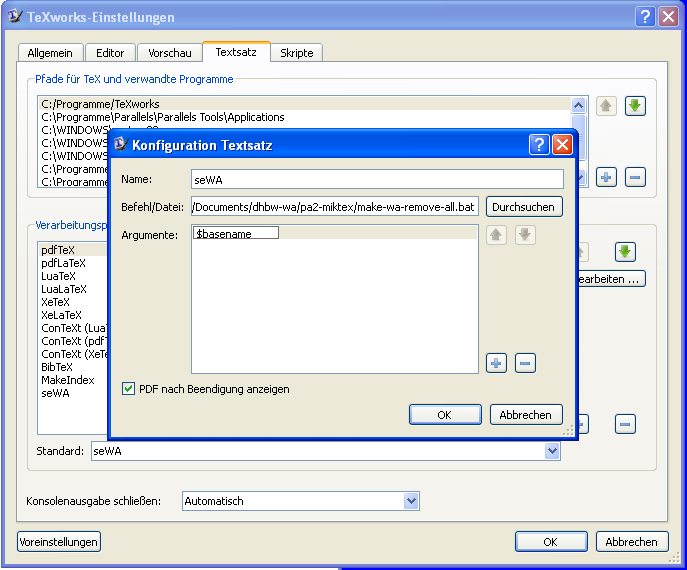
\includegraphics[width=\textwidth]{\seWaPathJpg/konfiguration-texworks.jpg}
\caption{Konfiguration von TeXworks -- Das Eintragen des Wertes  \texttt{\$basename} im Feld \textsl{Argumente}\label{texworks}}
\end{figure}

\newpage
\section{Ausdrucken des pdf-Dokuments}

Beim Ausdrucken des Dokuments (z. B. \"uber den Adobe Reader) muss unter \textsl{Seite anpassen} 
die Option \textsl{Tats\"achliche Gr\"o{\ss}e} ausgew\"ahlt werden (siehe \vref{ausdrucken}). Andernfalls werden die Einstellungen 
f\"ur das Layout der Arbeit nicht korrekt wiedergegeben. 

\begin{figure}[htbp]
\centering
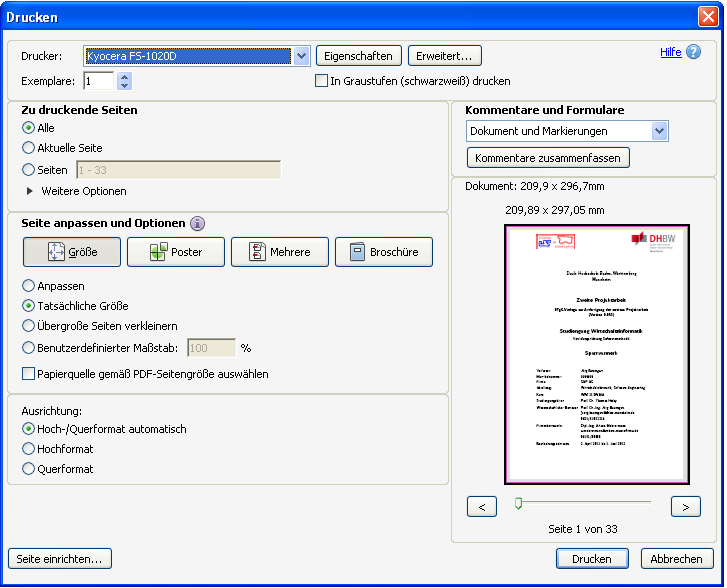
\includegraphics[width=\textwidth]{\seWaPathJpg/ausdrucken.jpg}
\caption{Ausdrucken des pdf-Dokuments -- Die Option \textsl{Tats\"achliche Gr\"o{\ss}e}\label{ausdrucken}}
\end{figure}




%Dann hoffe ich mal, dass sich mit den Vorlagen etwas anfangen lŠsst. Sie sind (absichtlich) in 
%
%einer Version 0.9, da ich an den zugehšrigen sty-Dateien weitere ErgŠnzungen vornehmen werde,
%
%um fŸr zukŸnftige Arbeiten neue komfortable Kommandos zur VerfŸgung zu stellen. 

\chapter{N\"utzliche \LaTeX-Pakete}

\section{bchart.sty -- Erstellung einfacher Balkendiagramme}

Das Paket \texttt{bchart} wurde von Tobias Kuhn entwickelt\seFootcite{Vgl.}{}{Kuh:Bch} und bietet die M\"oglichkeit, auf einfache Art und Weise \textbf{horizontale Balkendiagramme}
zu erzeugen.\footnote{Der Hinweis auf dieses Paket stammt von Julia Lakatos -- vielen Dank.} Weitere Informationen 
zur Anwendung des Pakets lassen sich bei dem \gls{ctan} finden.\footnote{\url{http://www.ctan.org/tex-archive/macros/latex/contrib/bchart}}
\vref{quelltext-bsp-bchart} enth\"alt den Quelltext f\"ur das Balkendiagramm aus \vref{bsp-bchart}.

\begin{programm}[htbp]
\begin{lstlisting}[keywordstyle=\color{black},showstringspaces=false]
\begin{figure}[htbp]
\centering
\begin{bchart}[step=10,max=100,width=11cm,unit=\,\%]
\bcbar[label=Note {1,0} -- {1,5}]{7.69}
\smallskip
\bcbar[label={1,6} -- {2,5}]{42.31}
\smallskip
\bcbar[label={2,6} -- {3,5}]{23.08}
\smallskip
\bcbar[label={3,6} -- {4,0}]{15.38}
\smallskip
\bcbar[label={4,1} -- {5,0}]{11.53}
\end{bchart}
\caption{Verteilung der Klausurnoten 
\textsl{Einf\"uhrung in die Programmierung}
\label{bsp-bchart}}
\end{figure}
\end{lstlisting}
\caption{Quelltext zur Erzeugung des Balkendiagramms aus \vref{bsp-bchart}\label{quelltext-bsp-bchart}}
\end{programm}
\clearpage


\begin{figure}[htbp]
\centering
\begin{bchart}[step=10,max=100,width=11cm,unit=\,\%]
\bcbar[label=Note {1,0} -- {1,5}]{7.69}
\smallskip
\bcbar[label={1,6} -- {2,5}]{42.31}
\smallskip
\bcbar[label={2,6} -- {3,5}]{23.08}
\smallskip
\bcbar[label={3,6} -- {4,0}]{15.38}
\smallskip
\bcbar[label={4,1} -- {5,0}]{11.53}
\end{bchart}
\caption{Verteilung der Klausurnoten 
\textsl{Einf\"uhrung in die Programmierung}
\label{bsp-bchart}}
\end{figure}


\newcommand{\TikZ}{\textsf{Ti\textsl{k}Z}}
\section{tikz.sty -- Konstruktion nahezu beliebig komplexer Grafiken}

Das \TikZ{}-Paket wurde urspr\"unglich von Till Tantau\seFootcite{Vgl.}{}{Tan:tik} entwickelt und erlaubt 
die Konstruktion nahezu beliebig komplexer Grafiken. 
Die Entwicklung des Pakets erfolgt derzeit auf SourceForge unter \url{http://sourceforge.net/projects/pgf}.\seFootcite{Vgl.}{}{Tan:tik}%
\seFootcite{Vgl.}{}{FT:tik}
Eine Einf\"uhrung in die Erstellung von Grafiken mit \TikZ{} ist in dem Buch von Joachim Schlosser zu 
finden.\seFootcite{Vgl.}{Kapitel 8.2.2, S. 138 ff}{Sch:WAS} Eine ausf\"uhrliche mehr als 700 Seiten umfassende Dokumentation wurde von Till Tantau in 
Zusammenarbeit mit weiteren Autoren verfasst.\seFootcite{Vgl.}{}{Tan:man}

\clearpage
\vref*{quelltext-bsp-tikz} enth\"alt den Quelltext f\"ur die Grafik aus \vref{bsp-tikz}.

\begin{programm}[htbp]
\begin{lstlisting}[showstringspaces=false]
\begin{figure}[htbp]
\centering
%
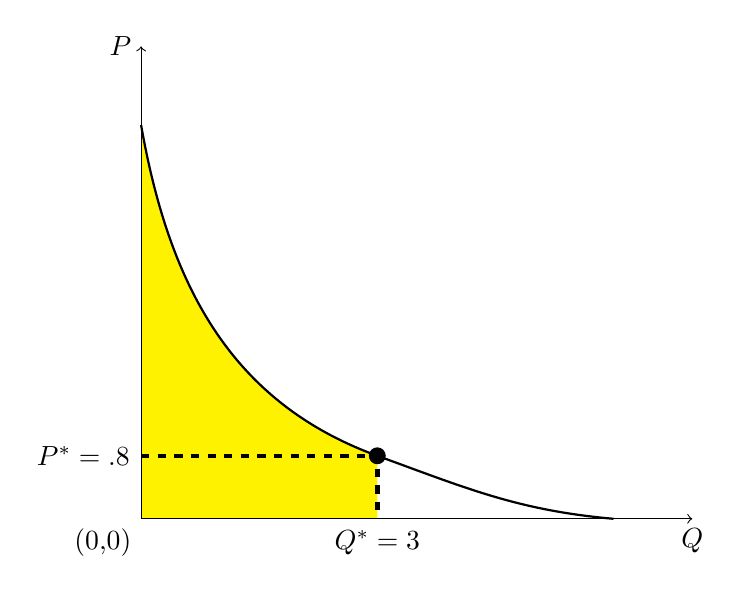
\begin{tikzpicture}
\path [fill=yellow] (0,0) -- (0,5) to [out=-80, in=160]
(3,.8) -- (3,0) -- (0,0);
\draw [<->] (0,6) node [left] {$P$} -- (0,0)
node [below left] {(0,0)} -- (7,0) node [below] {$Q$};
\draw [ultra thick, dashed] (0,.8) node [left] {$P^*=.8$} 
-- (3,.8) -- (3,0) node [below] {$Q^*=3$}; 
\draw [fill] (3,.8) circle (0.1);
\draw [thick] (0,5) to [out=-80, in=160] (3,.8) to
[out=-20, in=175] (6,0);
\end{tikzpicture}
%
\caption{Beispiel f\"ur eine mit \TikZ{} erstellte Grafik
\label{bsp-tikz}}
\end{figure}
\end{lstlisting}
\caption{Quelltext zur Erzeugung der Grafik aus \vref{bsp-tikz}\label{quelltext-bsp-tikz}}
\end{programm}



\begin{figure}[htbp]
\centering
%
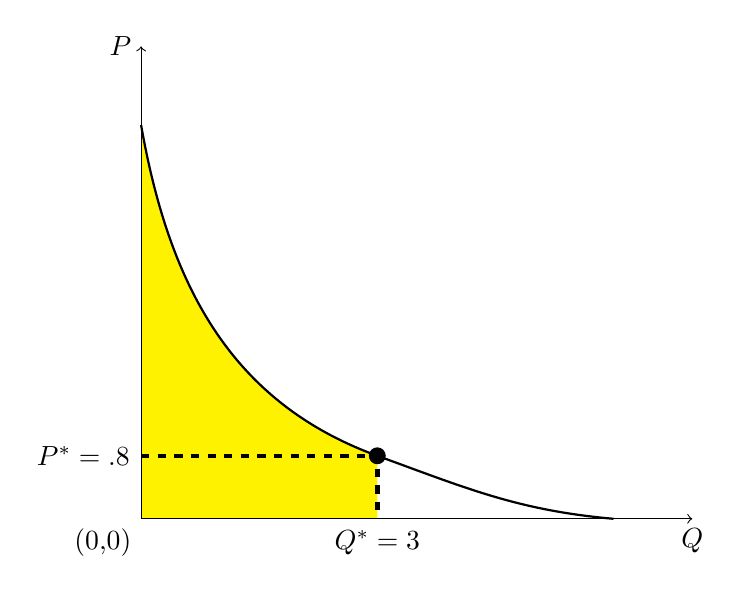
\begin{tikzpicture}
\path [fill=yellow] (0,0) -- (0,5) to [out=-80, in=160]
(3,.8) -- (3,0) -- (0,0);
\draw [<->] (0,6) node [left] {$P$} -- (0,0)
node [below left] {(0,0)} -- (7,0) node [below] {$Q$};
\draw [ultra thick, dashed] (0,.8) node [left] {$P^*=.8$} 
-- (3,.8) -- (3,0) node [below] {$Q^*=3$}; 
\draw [fill] (3,.8) circle (0.1);
\draw [thick] (0,5) to [out=-80, in=160] (3,.8) to
[out=-20, in=175] (6,0);
\end{tikzpicture}
%
\caption{Beispiel f\"ur eine mit \TikZ{} erstellte Grafik
\label{bsp-tikz}}
\end{figure}

\clearpage
\section{listings.sty -- Formatierung von Quelltexten}

Das Paket \texttt{listings.sty} wurde von Carsten Heinz und Brooks Moses entwickelt. Es unterst\"utzt f\"ur eine gro{\ss}e 
Menge von Programmiersprachen die Formatierung der Quelltexte.\seFootcite{Vgl.}{}{HM:lis} Die Liste der Sprachen reicht von 
ABAP bis XSLT.\seFootcite{Vgl.}{S. 12}{HM:lis}

Mit dem \texttt{lstset}-Kommando k\"onnen global f\"ur eine Programmiersprache die Formatierungsparameter definiert werden.
In \texttt{wa-konfiguration.tex} wurde beispielsweise festgelegt, dass standardm\"a{\ss}ig als Programmiersprache Java verwendet 
wird (\verb+language = Java+) und die Schl\"usselw\"orter blau darzustellen sind (\texttt{keywordstyle = \textbackslash{}color\{blue\}}).

F\"ur ein Listing lassen sich diese Eigenschaften \"uber optionale Parameter beim Start 
der \verb+lstlisting+-Umgebung umdefinieren. 


Bei \vref{bsp-zeilennummern} wurden statt \verb+\begin{lstlisting}+ einige optionale Parameter verwendet: \newline
\verb+\begin{lstlisting}[keywordstyle=\color{red},numbers=left,+\newline\verb+firstnumber=3,numbersep=5mm]+

\begin{seList}
\item \verb+firstnumber+ legt die erste Zeilennummer fest. Wird die Angabe von \verb+firstnumber+ weggelassen, 
dann wird der Standardwert 1 verwendet.
\item \verb+numbersep+ legt den Abstand zwischen der Zeilennummer und der ersten Spalte des Quelltextes fest. 
Fehlt die Angabe, dann wird der Standardwert 10pt benutzt.\seFootcite{Vgl.}{S. 31}{HM:lis}
\end{seList}

\begin{programm}[htbp]
\begin{lstlisting}[keywordstyle=\color{red},numbers=left,
firstnumber=3,numbersep=5mm]
public class HelloDHBW {
  public static void main ( String[] args ) {
    System.out.println ( "Hello DHBW" );
  } // main
} // HelloDHBW
\end{lstlisting}
\caption{Ausgabe eines Programms mit Zeilennummern und roten Schl\"usselw\"ortern\label{bsp-zeilennummern}}
\end{programm}

M\"ochte man verhindern, dass die Zeilennummern \"uber den linken Seitenrand hinausgehen, dann kann dieses mit 
dem optionalen Parameter \verb+xleftmargin+ erreicht werden. Beispielsweise liefert die zus\"atzliche Verwendung von 
\verb+xleftmargin=10mm+ die in \vref{bsp-leftmargin} dargestellte Formatierung.

\begin{programm}[htbp]
\begin{lstlisting}[numbers=left,
firstnumber=1,numbersep=5mm,xleftmargin=10mm]
public class HelloDHBW {
  public static void main ( String[] args ) {
    System.out.println ( "Hello DHBW" );
  } // main
} // HelloDHBW
\end{lstlisting}
\caption{Ausgabe eines Programms mit Zeilennummern sowie der 
Verwendung des optionalen Parameters \texttt{xleftmargin}\label{bsp-leftmargin}}
\end{programm}

Um f\"ur eine korrekte linksb\"undige Ausgabe der Zeilennummern nicht \textsl{\textbf{basteln}} zu m\"ussen, wird das neue 
Kommando \verb+\seListingLineNoConfig+ zur Verf\"ugung gestellt. Es besitzt vier Parameter:

\begin{seList}
\item Der erste Parameter ist (typischerweise) die \textbf{gr\"o{\ss}te Zeilennummer}, die in einem Listing auftritt. Hier\"uber wird die 
Breite ermittelt, die f\"ur die Zeilennummern ben\"otigt wird.\footnote{Prinzipiell reicht es aus, eine Zahl von 0 bis 9 anzugeben, wenn 
die gr\"o{\ss}te Zeilennummer einstellig ist, eine Zahl zwischen 10 und 99, wenn die gr\"o{\ss}te Zeilennummer zweistellig ist, usw.} Wenn f\"ur die 
Zeilennummern eine andere Schriftgr\"o{\ss}e oder eine spezielle Schriftart verwendet wird, dann sind die entsprechenden 
Schriftattribute ebenfalls mit anzugeben.
\item \"Uber den zweiten und dritten Parameter ist es m\"oglich, einen \textbf{Pr\"afix}- und \textbf{Postfixtext} f\"ur die Zeilennummern zu definieren. 
Beispielsweise k\"onnten die Zeilennummern in runde Klammern eingeschlossen werden. 
Wenn f\"ur die 
Zeilennummern eine andere Schriftgr\"o{\ss}e oder eine spezielle Schriftart verwendet wird, dann sind die entsprechenden 
Schriftattribute hier ebenfalls mit anzugeben.
\item Der vierte Parameter stellt den \textbf{Abstand zwischen der Zeilennummer und der ersten Spalte des Quelltextes} dar. Dieser Wert muss, 
um eine linksb\"undige Ausgabe der Zeilennummern zu erreichen, mit dem Wert \verb+numbersep+ \"ubereinstimmen.
\end{seList}

Mit dem Aufruf von \verb+\seListingLineNoConfig{13}{(}{)}{5mm}+ vor der Ausgabe des Quelltextes erreicht man die in \vref{bsp-linksbuendig} 
dargestellte Ausgabe der Zeilennummern, sofern bei \verb+\begin{lstlisting}+ gilt:

\begin{seList}
\item Der optionale Parameter \verb+firstnumber+ hat den Wert \verb+9+.
\item Der optionale Parameter \verb+numbersep+ hat den Wert \verb+5mm+.
\item Der optionale Paremeter \verb+xleftmargin+ hat den Wert \verb+\seListingLineNo+.\footnote{\texttt{\textbackslash{}seListingLineNo} wurde als 
\textsl{L\"angenregister} definiert. Das Kommando \texttt{\textbackslash{}se\-Lis\-ting\-Line\-No\-Con\-fig} berechnet den ben\"otigten Wert f\"ur \texttt{xleftmargin} und schreibt diesen 
Wert in das L\"angenregister.}
\end{seList}

\clearpage

\seListingLineNoConfig{13}{(}{)}{5mm}

\begin{programm}[htbp]
\begin{lstlisting}[numbers=left,firstnumber=9,numbersep=5mm,xleftmargin=\seListingLineNo]
public class HelloDHBW {
  public static void main ( String[] args ) {
    System.out.println ( "Hello DHBW" );
  } // main
} // HelloDHBW
\end{lstlisting}
\caption{Ausgabe eines Programms mit linksb\"undigen Zeilennummern\label{bsp-linksbuendig}}
\end{programm}


\section{supertabular.sty -- Mehrseitige Tabellen}

Das Paket \texttt{supertabular.sty} wurde von Johannes Braams und Theo Jurriens entwickelt.\seFootcite{Vgl.}{}{BJ:sup}
Neben der Erstellung mehrseitiger Tabellen bietet es im Vergleich zur \texttt{tabular}-Umgebung weitere Formatierungsm\"oglichkeiten.

Die wichtigsten Kommandos f\"ur mehrseitige Tabellen sind:\seFootcite{Vgl.}{S. 265}{MG:lat}

\begin{seList}
\item \texttt{\textbackslash{}tablehead\{{\textsl{zeilen}\}}} \newline
Der Parameter \textsl{zeilen} definiert die Tabellenzeilen, die am Kopf jeder Tabellenseite wiederholt werden.
\item \texttt{\textbackslash{}tablefirsthead\{{\textsl{zeilen}\}}} \newline
Wird neben \verb+tablehead+ auch \verb+tablefirsthead+ verwendet, so besteht die erste Tabellen\"uberschrift aus den 
Zeilen, die als Parameter \"uber \verb+\tablefirsthead+ festgelegt wurden. Auf allen Folgeseiten werden dann diejenigen 
Zeilen verwendet, die \"uber \verb+\tablehead+ definiert wurden.
\item \texttt{\textbackslash{}tabletail\{{\textsl{zeilen}\}}} \newline
Hiermit wird festgelegt, welche Zeilen am Ende einer Tabellenseite ausgegeben werden.
\item \texttt{\textbackslash{}tablelasttail\{{\textsl{zeilen}\}}} \newline
Mit \verb+\tablelasttail+ kann f\"ur die letzte Tabellenseite gesondert festgelegt werden, 
welche Zeilen auszugeben sind. 
\end{seList}

Die Angabe der Kommandos erfolgt vor der eigentlichen Verwendung der \texttt{su\-per\-ta\-bu\-lar}-Umgebung und wirkt sich auf alle 
folgenden Tabellen aus, die \"uber eine \texttt{su\-per\-ta\-bu\-lar}-Umgebung definiert werden. 

Da sich Gleitobjekte nicht \"uber mehrere Seiten erstrecken k\"onnen, ist es nicht sinnvoll, die \verb+supertabular+-Umgebung
mit der \verb+table+-Umgebung zu kombinieren. Um trotzdem eine Tabellenunterschrift erzeugen zu k\"onnen, stellt das 
\texttt{supertabular}-Paket eigene \verb+\caption+-Kommandos zur Verf\"ugung. Mit dem Kommando \texttt{\textbackslash{}bot\-tom\-cap\-tion} 
kann eine Tabellenunterschrift erzeugt werden, die auch in das Tabellenverzeichnis aufgenommen wird. Das \verb+\bottomcaption+-Kommando
muss ebenfalls vor dem Beginn der \verb+supertabular+-Umgebung angegeben werden.

In \vref{quelltext-bsp-supertabular} sind die Kommandos dargestellt, die f\"ur die Erzeugung der  \vref{bsp-supertabular} 
verwendet wurden. 

\begin{programm}[htbp]
\begin{lstlisting}[showstringspaces=false]
\tablefirsthead{\hline
   \multicolumn{2}{|c|}{\textbf{Gesamtumsatz 2012}}
   \\\hline\hline \textbf{Abteilung} 
   & \textbf{Umsatz}\\\hline}
\tablehead{\hline 
   \textbf{Abteilung} & \textbf{Umsatz}\\\hline}
\tabletail{\hline\multicolumn{2}{|r|}
   {\textsl{Fortsetzung n\"achste Seite}}\\\hline}
\tablelasttail{\hline
   \hline Gesamtumsatz & 148500,88\\\hline}
\bottomcaption{Jahresumsatz 2012\label{bsp-supertabular}}

\begin{center}%
\begin{supertabular}{ | l | r |}
Verkauf Industriemaschinen & 2100,55 \\
...
Verkauf 58 & 2100,55 \\
\end{supertabular}
\end{center}

\end{lstlisting}
\caption{Quelltext zur Erzeugung der \vref{bsp-supertabular}\label{quelltext-bsp-supertabular}}
\end{programm}

\tablefirsthead{\hline
   \multicolumn{2}{|c|}{\textbf{Gesamtumsatz 2012}}
   \\\hline\hline \textbf{Abteilung} 
   & \textbf{Umsatz}\\\hline}
\tablehead{\hline 
   \textbf{Abteilung} & \textbf{Umsatz}\\\hline}
\tabletail{\hline\multicolumn{2}{|r|}
   {\textsl{Fortsetzung n\"achste Seite}}\\\hline}
\tablelasttail{\hline
   \hline Gesamtumsatz & 148500,88\\\hline}
\bottomcaption{Jahresumsatz 2012\label{bsp-supertabular}}


%\tablefirsthead{\hline\multicolumn{2}{|c|}{\textbf{Gesamtumsatz 2012}}\\\hline\hline \textbf{Abteilung} & \textbf{Umsatz}\\\hline}
%\tablehead{\hline \textbf{Abteilung} & \textbf{Umsatz}\\\hline}
%\tabletail{\hline\multicolumn{2}{|r|}{\textsl{Fortsetzung n\"achste Seite}}\\\hline}
%\tablelasttail{\hline\hline Gesamtumsatz & 148500,88\\\hline}
%\bottomcaption{Jahresumsatz 2012\label{bsp-supertabular}}

\begin{center}%
\begin{supertabular}{ | l | r |}
Verkauf Industriemaschinen & 2100,55 \\
Verkauf 1 & 3020,17 \\
Verkauf 2 & 2100,55 \\
Verkauf 3 & 3020,17 \\
Verkauf 4 & 2100,55 \\
Verkauf 5 & 3020,17 \\
Verkauf 6 & 2100,55 \\
Verkauf 7 & 3020,17 \\
Verkauf 8 & 3020,17 \\
Verkauf 9 & 2100,55 \\
Verkauf 10 & 3020,17 \\
Verkauf 11 & 2100,55 \\
Verkauf 12 & 3020,17 \\
Verkauf 13 & 2100,55 \\
Verkauf 14 & 3020,17 \\
Verkauf 15 & 2100,55 \\
Verkauf 16 & 3020,17 \\
Verkauf 17 & 2100,55 \\
Verkauf 18 & 3020,17 \\
Verkauf 19 & 3020,17 \\
Verkauf 20 & 2100,55 \\
Verkauf 21 & 3020,17 \\
Verkauf 22 & 2100,55 \\
Verkauf 23 & 3020,17 \\
Verkauf 24 & 2100,55 \\
Verkauf 25 & 3020,17 \\
Verkauf 26 & 2100,55 \\
Verkauf 27 & 3020,17 \\
Verkauf 28 & 2100,55 \\
Verkauf 29 & 3020,17 \\
Verkauf 30 & 2100,55 \\
Verkauf 31 & 3020,17 \\
Verkauf 32 & 2100,55 \\
Verkauf 33 & 3020,17 \\
Verkauf 34 & 2100,55 \\
Verkauf 35 & 3020,17 \\
Verkauf 36 & 2100,55 \\
Verkauf 37 & 3020,17 \\
Verkauf 38 & 3020,17 \\
Verkauf 39 & 2100,55 \\
Verkauf 40 & 3020,17 \\
Verkauf 41 & 2100,55 \\
Verkauf 42 & 3020,17 \\
Verkauf 43 & 2100,55 \\
Verkauf 44 & 3020,17 \\
Verkauf 45 & 2100,55 \\
Verkauf 46 & 3020,17 \\
Verkauf 47 & 2100,55 \\
Verkauf 48 & 3020,17 \\
Verkauf 49 & 3020,17 \\
Verkauf 50 & 2100,55 \\
Verkauf 51 & 3020,17 \\
Verkauf 52 & 2100,55 \\
Verkauf 53 & 3020,17 \\
Verkauf 54 & 2100,55 \\
Verkauf 55 & 3020,17 \\
Verkauf 56 & 2100,55 \\
Verkauf 57 & 3020,17 \\
Verkauf 58 & 2100,55 \\
\end{supertabular}
\end{center}


\section{algorithm2e.sty -- Spezifikation von Algorithmen}

Das Paket \texttt{algorithm2e} wurde von Christophe Fiorio entwickelt.\seFootcite{Vgl.}{}{Fio:alg}
Das Paket unterst\"utzt die Spezifikation von Algorithmen und stellt zahlreiche Optionen 
f\"ur das Layout zur Verf\"ugung.\footnote{Der Hinweis auf dieses Paket stammt von Jan Schlenker -- vielen Dank.}
Das aktuelle Release 5.0 vom 6. Januar 2013 ist im Verzeichnis \verb+se-wa-styles+ zu finden.

Um f\"ur Algorithmen ein eigenes Algorithmenverzeichnis erstellen zu k\"onnen, wird die neue Umgebung \verb+algorithmus+ 
bereitgestellt. Zus\"atzlich wurde das Kommando \verb+\seVerzeichnisse+ f\"ur die Ausgabe des Algorithmenverzeichnisses 
um einen siebten Parameter erg\"anzt.

\vref*{alg1-quelltext} enth\"alt die Kommandos f\"ur die Spezifikation des \vref{alg1}.

\clearpage
\begin{programm}[htbp]
\begin{lstlisting}[keywordstyle=\color{black}]
\begin{algorithmus}[htbp]
\begin{algorithm}[H]
  \KwData{this text}
  \KwResult{how to write algorithm with \LaTeX2e }
  
  initialization\;
  \While{not at end of this document}{
    read current\;
    \eIf{understand}{
      go to next section\;
      current section becomes this one\;
      }{
      go back to the beginning of current section\;
      }
    }
\end{algorithm}
\caption{How to write algorithms}
\end{algorithmus}
\end{lstlisting}
\caption{Quelltext zur Spezifikation des \vref{alg1}\label{alg1-quelltext}}
\end{programm}

\vspace{\baselineskip}
\begin{algorithmus}[htbp]
\begin{algorithm}[H]  \KwData{this text}
  \KwResult{how to write algorithm with \LaTeX2e }
  
  initialization\;
  \While{not at end of this document}{
    read current\;
    \eIf{understand}{
      go to next section\;
      current section becomes this one\;
      }{
      go back to the beginning of current section\;
      }
    }
\end{algorithm}
\caption{How to write algorithms\label{alg1}}
\end{algorithmus}

Wichtig ist, bei dem Kommando \verb+\begin{algorithm}[H]+ den optionalen Parameter \verb+[H]+ anzugeben. Ohne 
diesen Parameter erzeugt die \"Ubersetzung des Dokuments die Fehlermeldung \glqq{}\verb+! LaTeX Error: Not in outer par mode+\grqq{}.

Beim Laden des Paketes k\"onnen verschiedene Optionen angegeben werden.\seFootcite{Vgl.}{S.\,18--20 }{Fio:alg} Das vorliegende Layout wurde 
durch die Anweisung \newline\hspace*{\fill}\verb+\usepackage[boxed,ngerman]{algorithm2e}+\hspace*{\fill}\newline erreicht.%
\footnote{Die zugeh\"orige \texttt{\textbackslash{}usepackage-Anweisung} ist in der Datei \waInputStyles{} im 
Verzeichnis  \texttt{se-wa-styles} zu finden, wobei \texttt{\textbackslash{}seWaPathSty} das Verzeichnis definiert, in dem die 
\texttt{.sty}-Dateien liegen.} Verwendet man stattdessen die Anweisung 
\newline\hspace*{\fill}\verb+\usepackage[tworuled,vlined,ngerman]{algorithm2e}+\hspace*{\fill}\newline wird das Layout erzeugt, 
das in \vref{alg2} zu sehen ist. Um bei der Anwendung der \verb+tworuled+- oder \verb+plain+-Option eine linksb\"undige Ausgabe des 
Algorithmus zu erreichen, muss zus\"atzlich das Kommando \newline\hspace*{\fill}\verb+\setlength{\algomargin}{0mm}+\hspace*{\fill}\newline benutzt werden.

\begin{programm}[htbp]
\begin{lstlisting}[keywordstyle=\color{black}]
\begin{algorithmus}[htbp]
\IncMargin{1cm}
\begin{algorithm}[H]
\DontPrintSemicolon
\KwData{$G=(X,U)$ such that $G^{tc}$ is an order.}
\KwResult{$G'=(X,V)$ with $V\subseteq U$ such that $G'^{tc}$ is an
interval order.}
\Begin{
  $V \longleftarrow U$\;
  $S \longleftarrow \emptyset$\; 
  \For{$x\in X$}{ 
    $NbSuccInS(x) \longleftarrow 0$\;
    $NbPredInMin(x) \longleftarrow 0$\;
    $NbPredNotInMin(x) \longleftarrow |ImPred(x)|$\;
    }
  \For{$x \in X$}{
    \If{$NbPredInMin(x) = 0$ {\bf and} $NbPredNotInMin(x) = 0$}{
      $AppendToMin(x)$}
    } 
    \nl\While{$S \neq \emptyset$}{\label{InRes1}
    \nlset{REM} remove $x$ from the list of $T$ of maximal index\;\label{InResR}
    \lnl{InRes2}\While{$|S \cap  ImSucc(x)| \neq |S|$}{ 
      \For{$ y \in  S-ImSucc(x)$}{
        \{ remove from $V$ all the arcs $zy$ : \}\;
        \For{$z \in  ImPred(y) \cap  Min$}{
          remove the arc $zy$ from $V$\;
          $NbSuccInS(z) \longleftarrow NbSuccInS(z) - 1$\;
          move $z$ in $T$ to the list preceding its present list\;
          \{i.e. If $z \in T[k]$, move $z$ from $T[k]$ to 
           $T[k-1]$\}\;
          }
        $NbPredInMin(y) \longleftarrow 0$\;
        $NbPredNotInMin(y) \longleftarrow 0$\;
        $S \longleftarrow S - \{y\}$\;
        $AppendToMin(y)$\;
        }
      }
    $RemoveFromMin(x)$\;
    }
  }  
%\caption{IntervalRestriction\label{IR}}
\end{algorithm}

\vspace*{-2mm}
\caption{Der Formatierung des Algorithmus 
         IntervalRestriction unter Verwendung von 
         \texttt{\textbackslash{}IncMargin\{1cm\}} 
         und \texttt{\textbackslash{vspace*\{-2mm\}}}
         \label{alg2}}
\end{algorithmus}
\end{lstlisting}
\caption{Quelltext zur Spezifikation des \vref{alg2}\label{alg2-quelltext}}
\end{programm}



% Die beiden folgenden Anweisungen dienen als Alternative, um ein Layout zu erzeugen, das 
% \usepackage[tworuled,vlined,ngerman]{\seWaPathSty/algorithm2e} entspricht.
\RestyleAlgo{tworuled}
\SetAlgoVlined{}

\setlength{\algomargin}{0mm}



Das Kommando \verb+\IncMargin{1cm}+ hat eine Einr\"uckung des Algorithmus um 1\,cm zur Folge. Diese ist 
notwendig, da andernfalls durch die Verwendung der \textsc{rem}-Markierung der Algorithmus \"uber den 
linken Seitenrand hinausgeht. Ein \verb+\vspace*+-Kommando kann verwendet werden, um den Abstand 
zwischen dem Algorithmus und der Algorithmusunterschrift (erzeugt durch das \verb+\caption+-Kommando) zu ver\"andern.

\clearpage
\begin{algorithmus}[htbp]
\IncMargin{1cm}
\begin{algorithm}[H]
\DontPrintSemicolon
\KwData{$G=(X,U)$ such that $G^{tc}$ is an order.}
\KwResult{$G'=(X,V)$ with $V\subseteq U$ such that $G'^{tc}$ is an
interval order.}
\Begin{
  $V \longleftarrow U$\;
  $S \longleftarrow \emptyset$\; 
  \For{$x\in X$}{ 
    $NbSuccInS(x) \longleftarrow 0$\;
    $NbPredInMin(x) \longleftarrow 0$\;
    $NbPredNotInMin(x) \longleftarrow |ImPred(x)|$\;
    }
  \For{$x \in X$}{
    \If{$NbPredInMin(x) = 0$ {\bf and} $NbPredNotInMin(x) = 0$}{
      $AppendToMin(x)$}
    } 
    \nl\While{$S \neq \emptyset$}{\label{InRes1}
    \nlset{REM} remove $x$ from the list of $T$ of maximal index\;\label{InResR}
    \lnl{InRes2}\While{$|S \cap  ImSucc(x)| \neq |S|$}{ 
      \For{$ y \in  S-ImSucc(x)$}{
        \{ remove from $V$ all the arcs $zy$ : \}\;
        \For{$z \in  ImPred(y) \cap  Min$}{
          remove the arc $zy$ from $V$\;
          $NbSuccInS(z) \longleftarrow NbSuccInS(z) - 1$\;
          move $z$ in $T$ to the list preceding its present list\;
          \{i.e. If $z \in T[k]$, move $z$ from $T[k]$ to 
           $T[k-1]$\}\;
          }
        $NbPredInMin(y) \longleftarrow 0$\;
        $NbPredNotInMin(y) \longleftarrow 0$\;
        $S \longleftarrow S - \{y\}$\;
        $AppendToMin(y)$\;
        }
      }
    $RemoveFromMin(x)$\;
    }
  }  
%\caption{IntervalRestriction\label{IR}}
\end{algorithm}

\vspace*{-2mm}
\caption{Der Formatierung des Algorithmus 
         IntervalRestriction unter Verwendung von 
         \texttt{\textbackslash{}IncMargin\{1cm\}} 
         und \texttt{\textbackslash{vspace*\{-2mm\}}}
         \label{alg2}}
\end{algorithmus}



\chapter{Tipps und Tricks}

\section{Verwendung einer Listenumgebung in einer Tabelle}

Um z.\,B. die \verb+seList+-Umgebung in einer Tabelle verwenden zu k\"onnen, ist es notwendig, die Liste 
in eine \verb+\parbox+ zu integrieren, da andernfalls die \"Ubersetzung des Dokumentes mit einer 
Fehlermeldung abgebrochen wird. 

\vref*{quelltext-tab-ereignisse} enth\"alt den Quelltext f\"ur die \vref{tab-ereignisse}. Da das Kommando 
\newline\hspace*{\fill}\verb+\seSetlistbaselineskip+\hspace*{\fill}\newline in einer 
\verb+\parbox+ nicht funktioniert, muss das \textbf{Spacing} der Listeneintr\"age per Hand durch entsprechende
\verb+\vspace*+-Kommandos vorgenommen werden.
 
\vspace{\baselineskip}
\begin{table}[htbp]
\centering
\begin{tabular}{| c | c |}
\hline
Ereignis & Eventuelle Folgen/Kommentar \\
\hline
Konjunkturkrise &
\parbox[t]{6cm}{%
\begin{seList}
\vspace*{-0.55\baselineskip}
\item Produktionsverminderung
\vspace*{-0.5\baselineskip}
\item Entlassung von Mitarbeitern
\vspace*{-0.5\baselineskip}
\item Es ist aber in der Regel keine gute Idee, sich von
hochqualifizierten Mitarbeitern zu trennen
\vspace*{0.25\baselineskip}
\end{seList}
} % \parbox
\\
\hline
\end{tabular}
\caption{Ereignisse und ihre Folgen\label{tab-ereignisse}}
\end{table} 
 

\clearpage
\begin{programm}[htbp]
\begin{lstlisting}[keywordstyle=\color{black}]
\begin{table}[htbp]
\centering
\begin{tabular}{| c | c |}
\hline
Ereignis & Eventuelle Folgen/Kommentar \\
\hline
Konjunkturkrise &
\parbox[t]{6cm}{%
\begin{seList}
\vspace*{-0.55\baselineskip}
\item Produktionsverminderung
\vspace*{-0.5\baselineskip}
\item Entlassung von Mitarbeitern
\vspace*{-0.5\baselineskip}
\item Es ist aber in der Regel keine gute Idee, sich von
hochqualifizierten Mitarbeitern zu trennen
\vspace*{0.25\baselineskip}
\end{seList}
} % \parbox
\\
\hline
\end{tabular}
\caption{Ereignisse und ihre Folgen\label{tab-ereignisse}}
\end{table} 
\end{lstlisting}
\caption{Der Quelltext f\"ur die \vref{tab-ereignisse}\label{quelltext-tab-ereignisse}}
\end{programm}

\newpage
\section{Mehrseitige Listings}

Wenn die \verb+programm+-Umgebung verwendet wird, ist es nicht m\"oglich, mehrseitige 
Listings zu erzeugen.\footnote{Dies liegt in der Tatsache begr\"undet, dass sich Gleitobjekte (floats) nicht \"uber mehrere Seiten 
erstrecken k\"onnen.} 
Benutzt man die \verb+lstlisting+-Umgebung ohne die \verb+programm+-Umgebung, k\"onnen zwar einerseits mehrseitige Listings 
erzeugt werden, andererseits ist es aber auf direktem Weg nicht m\"oglich, die Listingunterschrift in das Listingverzeichnis aufzunehmen.%
\footnote{Von der Verwendung des \texttt{\textbackslash{}lstlistoflistings}-Kommandos wird \textbf{dringend abgeraten}, da es keine Kontrolle \"uber 
das Layout des Listings-Verzeichnisses erlaubt und nicht zum Layout der anderen Verzeichnisse passt.} 

Eine L\"osung f\"ur diese Problematik stellt das
neue Kommando \verb+\captionListing+ dar. Es besitzt einen Parameter, der den Wert f\"ur das ebenfalls neue Kommando \verb+\captionListingText+ 
definiert. Das \verb+\captionListing+-Kommando muss direkt vor einer Verwendung der \verb+lstlisting+-Umgebung angegeben werden. Es sorgt unter anderem 
daf\"ur, dass die \"uber \verb+\captionListingText+ definierte Listingunterschrift in das Listingverzeichnis aufgenommen wird.

Das \vref{lis-mehrseitig} wird durch den Quelltext aus \vref{quelltext-lis-mehrseitig} erzeugt.


\captionListing{Beispiel f\"ur ein mehrseitiges Listing}
\begin{lstlisting}[caption=\captionListingText,
       label=lis-mehrseitig,
       abovecaptionskip=3mm,aboveskip=\parskip]
zeile 01;
zeile 02;
zeile 03;
zeile 04;
zeile 05;
zeile 06;
zeile 07;
zeile 08;
zeile 09;
zeile 10;
zeile 11;
zeile 12;
zeile 13;
zeile 14;
zeile 15;
zeile 16;
zeile 17;
zeile 18;
zeile 19;
zeile 20;
zeile 21;
zeile 22;
zeile 23;
zeile 24;
\end{lstlisting}

\vspace*{\baselineskip}
\begin{programm}[htbp]
\begin{verbatim}
\captionListing{Beispiel f\"ur ein mehrseitiges Listing}
\begin{lstlisting}[caption=\captionListingText,
       label=lis-mehrseitig,
       abovecaptionskip=3mm,aboveskip=\parskip]
zeile 01;
zeile 02;
zeile 03;
zeile 04;
zeile 05;
zeile 06;
zeile 07;
zeile 08;
zeile 09;
zeile 10;
zeile 11;
zeile 12;
zeile 13;
zeile 14;
zeile 15;
zeile 16;
zeile 17;
zeile 18;
zeile 19;
zeile 20;
zeile 21;
zeile 22;
zeile 23;
zeile 24;
\end{lstlisting}
\end{verbatim}
\vspace*{-3.5mm}
\caption{Quelltext von \vref{lis-mehrseitig}\label{quelltext-lis-mehrseitig}}
\end{programm}

\clearpage
Die optionalen Parameter der \verb+lstlisting+-Umgebung haben hierbei die folgende Bedeutung:

\begin{seList}
\item \verb+caption=\captionListingText+

Festlegung der Listingunterschrift; hierf\"ur sollte grunds\"atzlich das Kommando \verb+\captionListingText+ verwendet werden.

\item \verb+label=lis-mehrseitig+

Definition eines Labels, mit dem sp\"ater, z.\,B. \"uber das \verb+\vref+-Kommando, auf die Listingnummer zugegriffen werden kann. \newline 
Dies entspricht dem \verb+\label{}+-Kommando, das beispielsweise bei einer \verb+programm+-Umgebung verwendet wird.

\item \verb+abovecaptionskip=3mm+

Definition eines zus\"atzlichen Abstands zwischen dem eigentlichen Listing und der Listingunterschrift.

\item \verb+aboveskip=\parskip+ 

Vor dem Listing wird ein zus\"atzlicher Abstand erzeugt, der dem Abstand zwischen zwei Abs\"atzen entspricht.
\end{seList}

Durch die Verwendung des \verb+\captionListing+-Kommandos wird sichergestellt, dass die \verb+lstlisting+-Umgebung und die 
\verb+programm+-Umgebung gemeinsam in einem Dokument verwendet werden k\"onnen.



\chapter{Literaturempfehlungen}

\begin{seList}
\item \textsl{Schlosser: Wissenschaftlich Arbeiten mit \LaTeX -- Leitfaden f\"ur Einsteiger}\seFootcite{}{}{Sch:WAS4}\newline
Dieses Buch bietet eine sehr gute, kompakte Einf\"uhrung in \LaTeX. Es enth\"alt Informationen zu 
aktuellen Paketen. 
\item \textsl{Mittelbach/Goossens: Der LaTeX-Begleiter}\seFootcite{}{}{MG:lat}\newline
Das Buch hat einen Umfag von 1138 Seiten und geht ausf\"uhrlich auf eine Vielzahl von Paketen ein. 
Zus\"atzlich werden grundlegende Konzepte vorgestellt, die einen Einblick in die Struktur des \LaTeX-Systems bieten.
Es ist allerdings kein Buch f\"ur einen schnellen Einstieg in \LaTeX, sondern als Nachschlagewerk f\"ur viele Fragen 
rund um das Thema \LaTeX{} gedacht.
\item \textsl{Kohm/Morawski: KOMA-Script -- Eine Sammlung von Klassen und Paketen f\"ur \LaTeXe}\seFootcite{}{}{KM:KS4}\newline
Das Buch stellt ausf\"uhrlich die KOMA-Script-Klassen f\"ur die Erstellung von B\"uchern, Reports, Artikeln und Briefen vor, 
die explizit die Regeln der europ\"aischen Typographie unterst\"utzen. Diese Klassen enthalten sehr viele Parameter, \"uber die 
sich das grundlegende Layout vergleichsweise komfortabel steuern l\"asst. Die KOMA-Script-Klasse \texttt{scrreprt} bildet die 
Grundlage f\"ur die Vorlagendateien zur Erstellung von Seminar-, Projekt- und Bachelorarbeiten.
\item \textsl{Lingnau: \LaTeX-Hacks -- Tipps \& Techniken f\"ur professionellen Textsatz}\seFootcite{}{}{Lin:lat}\newline
Das Buch enth\"alt eine Sammlung von Tricks, Methoden und Techniken aus den vielf\"altigen Anwendungsbereichen von 
\LaTeX{} und \TeX. Bei der Auswahl der Hacks wurde besonderes Augenmerk auf kreative L\"osungen gelegt, die mit 
\LaTeX{} m\"oglich sind.\seFootcite{Vgl.}{Klappentext}{Lin:lat}
\end{seList}

\chapter{Hinweise zum Literaturverzeichnis}

Im Literaturverzeichnis dieses Dokuments sind deutlich mehr Quellen angegeben als im 
Text verwendet wurden. Dies widerspricht der Regel, dass in einem Literaturverzeichnis 
nur diejenigen Quellen aufgef\"uhrt werden, die auch in der (wissenschaftlichen) Arbeit 
referenziert wurden. 

Bei der Erstellung dieses Literaturverzeichnisses wurde jedoch das Ziel verfolgt, 
m\"oglichst viele unterschiedliche Beispiele f\"ur Quellenangaben vorzustellen. 
Die zugeh\"origen Definitionen sind in der Datei \texttt{wa.bib} zu finden und 
k\"onnen als Vorlage f\"ur die Erstellung eigener \texttt{.bib}-Dateien verwendet 
werden. 


%
%  Erzeugung eines Glossars
%
% Achtung: Das Glossar wird nur ausgegeben, wenn mindestens ein Eintrag in der Arbeit
%                definiert wurde
%
%

% Die folgenden Kapitel beginnen jeweils auf einer neuen Seite
%
%
\seChaptersNewpage{}
%\newpage
\sePrintGlossary{}


%
% Literaturverzeichnisses
%
%\newpage
\sePrintBibliography{}

%  Erzeugung von Eintr\"agen im Literaturverzeichnis
%
%  Achtung: in einer Seminar-/Projekt/Bachelorarbeit darf da \nocite-Kommando nicht verwendet werden,
%                 da es einen Eintrag im Literaturverzeichnis erzeugt, ohne dass eine
%                 entsprechende Literaturreferenz im Text der Arbeit angegeben wird
%
%
%
%\nocite{DHBW:SG}
%\nocite{KM:KS}
%\nocite{Dud06}
%\nocite{Dud09}
%\nocite{Bri:WA}
%\nocite{RP:WA}
%\nocite{Sch:WAS}
%\nocite{BSS:WA}
%\nocite{Kor:WA}
%\nocite{MK:GWA}
%\nocite{ADG:WA}
%\nocite{The:WA}
%\nocite{BA:WA}
%\nocite{Dij:CRT}
%\nocite{BC:Cur}
%\nocite{Par:ECP}
%\nocite{Bro:SBE}
%\nocite{GI:ADI}
%\nocite{GI:AZI}
%\nocite{Den:CD}
%\nocite{LMS:Icb}
%\nocite{Fre:SIF}



%
% Festlegung des grundlegenden Formatierungsstils des Literaturverzeichnis
%
\bibliographystyle{jurabib}

% Eigentliche Ausgabe der in der Arbeit verwendeten Quellen
%
%
% Angabe der bib-Dateien, in denen die Quellen beschrieben sind;
% die Angabe geht davon aus, dass eine wa.bib-Datei in demselben
% Verzeichnis liegt, wie se-ba-vorlage.tex
%

% 2012-02-06
%
% Umbenennung von Literatur- in Quellenverzeichnis
%
%\renewcommand*{\bibname}{Quellenverzeichnis}
\seBibliography{wa}


%
% Erzeugung der ehrenw\"ortlichen Erkl\"arung
%
% Der optionale Parameter kann verwendet werden, um f\"ur das Thema der Arbeit eine
% andere Formatierung vorzunehmen; das sollte in der Regel nicht erforderlich sein;
% ausserdem besteht die Gefahr inkonsistenter Titel auf dem Titelblatt und in der
% ehrenw\"ortlichen Erkl\"arung
%
\seEhrenwoertlicheErklaerung{} % dieses Kommando sollte standardm\"assig verwendet werden
%\seEhrenwoertlicheErklaerung[\LaTeX-Vorlage zur Anfertigung einer Seminararbeit (Version \version{})]


\end{document}
